\section{Design of \sys}

In this section, we describe the design of \sys, which assesses vulnerability exploitability by identifying the configuration context under which a given PoC can trigger the vulnerable behavior in a downstream application.

\PP{Overview}
\autoref{fig:overview} shows the three-phase workflow of \sys: P1 for \textit{vulnerability-relevant state identification}, P2 for \textit{downstream configuration recovery}, and P3 for \textit{trigger synthesis}. \sys assesses downstream exploitability by analyzing the upstream and downstream components separately and connecting them across the component boundary. 
%\sys assesses downstream exploitability by separately analyzing the upstream and downstream components and connecting the resulting information across their boundary. \autoref{fig:overview} shows the high-level workflow of \sys, which comprises three phases: 

% Assessing downstream exploitability requires reasoning about both the upstream and downstream components. However, jointly analyzing their executions is costly and complex. To address this, \sys analyzes the two components separately and connects the resulting information across the component boundary.

% Assessing exploitability under a downstream configuration context requires analyzing both the upstream and downstream components. However, jointly analyzing their executions is costly and complex. To address this, \sys analyzes the two components separately and connects the resulting information across the component boundary.

%\autoref{fig:overview} shows the high-level workflow of \sys, which comprises three phases: 

% \vspace{2px}
% \textbf{P1.} Vulnerability-relevant state identification
% \vspace{1px}

% \textbf{P2.} Downstream configuration recovery
% \vspace{1px}

% \textbf{P3.} Trigger synthesis
% \vspace{2px}


In P1, \sys analyzes the upstream component to identify the vulnerability-relevant state consumed along the vulnerable path. In P2, it recovers how the downstream application can influence this state, including the corresponding operations, execution paths, and controllable interfaces. Together, P1 and P2 address the cross-boundary configuration challenge (\autoref{subsec:moti}) by connecting downstream configuration to vulnerability-relevant upstream state.
%
In P3, \sys synthesizes an executable test harness, searches for concrete interface values, and validates whether the recovered configuration can trigger the vulnerability. This addresses the execution-feasibility challenge by concretely exercising the recovered
downstream execution with the given PoC.


% In P1, \sys analyzes the upstream component to identify the vulnerability-relevant state consumed along the vulnerable path. In P2, \sys analyzes the downstream application to recover how that state can be established or influenced, including the corresponding operations, execution paths, and externally controllable interfaces. Together, P1 and P2 address the cross-boundary configuration challenge (\autoref{subsubsec:chall}) by connecting
% downstream-controlled configuration to the upstream state that affects the vulnerability.

% Finally, in P3, \sys combines these results to synthesize an executable test harness, search for concrete interface values, and validate whether the downstream application can trigger the vulnerability. This addresses the execution-feasibility challenge by concretely exercising the recovered configuration along a downstream execution that delivers the PoC to the vulnerable upstream behavior.

% In P1, \sys analyzes the upstream component to identify the
% vulnerability-relevant state consumed along the vulnerable path. In P2, \sys analyzes the downstream application to recover how that state can be established or influenced, including the corresponding operations, execution paths, and externally controllable interfaces. Finally, in P3, \sys combines these results to synthesize an executable test harness, search for concrete interface values, and validate whether the downstream application can trigger the vulnerability.

% Given an upstream component, a downstream application, and a valid PoC, in P1, \sys traces execution from the boundary APIs to the vulnerability and identifies the memory locations whose values are consumed along the vulnerable path. In P2, \sys connects these locations to downstream operations through abstract-location matching, classifies how the downstream application can influence them, and recovers the corresponding execution sequences and externally controllable interfaces. Finally, in P3, \sys translates the recovered information into an executable test harness, searches for concrete values for the recovered interfaces, and validates whether they trigger the vulnerability under the given PoC.

% In P1, \sys uses \textit{static dependency analysis} and \textit{abstract-location joining} to identify the downstream configuration context required to trigger the upstream vulnerability.
% It outputs a set of facts describing how the downstream application establishes this configuration, including its state, the APIs that manipulate it, and the execution paths that reach it.
% In P2, \sys \textit{generates a harness}---a driver program that invokes $D$'s public interface to reproduce the fault---from the P1 output and uses \textit{targeted symbolic execution} to derive concrete runtime settings that trigger the vulnerability under $P$.
% The output of P2 is a configuration assignment that realizes $C_C$.



% \begin{figure}[t]
%   \centering
%   \includegraphics[width=1\linewidth]{./imgs/overview_HJ.pdf}
%   \caption{Overview of \sys.}
%   \label{fig:overview}
% \end{figure}


\subsection{Vulnerability-Relevant State Identification}
\label{subsec:p1}

Given the upstream component $U$, the downstream application $D$, and
the fault location reported for the given PoC, \sys identifies the
upstream state that affects vulnerability triggering. To do so, it analyzes the
intermediate representation (IR) of $U$ to recover the vulnerable
execution and identify the memory locations consumed along its path.

%Given the upstream component $U$, the downstream application $D$, and the fault location reported for the given PoC, \sys identifies the vulnerability-relevant state in $U$. \sys analyzes the intermediate representation (IR) of $U$ to locate the vulnerable execution and identify memory locations whose values are consumed along its path.

%Given the upstream component $U$, the downstream application $D$, and the vulnerability sink identified from the given PoC, \sys identifies the vulnerability-relevant state in $U$. \sys analyzes the intermediate representation (IR) of $U$ to identify memory locations consumed along the vulnerable execution and represents them as abstract memory locations. %These locations are passed to P2 to recover the corresponding downstream configuration.

% Given the upstream component $U$, the downstream application $D$, and the vulnerability sink identified from the given PoC, \sys first identifies the \textit{vulnerability-relevant state} in $U$. We use this term to refer to memory locations whose values are consumed along the execution leading to the vulnerability. The identified state is then used by P2 to recover the corresponding downstream configuration.

%\noindent\textbf{Phase overview.}
% Given the upstream component $U$, the downstream application $D$, and the vulnerability sink identified from the given PoC, \sys first identifies the runtime state in $U$ that may influence the vulnerable execution.

% To this end, P1 identifies the boundary APIs through which $D$ invokes $U$, recovers the upstream paths from these APIs to the vulnerability, and collects the memory state consumed along those paths. It then represents the identified state as abstract memory locations, which are used by P2 to recover the corresponding downstream configuration.

% To this end, \sys analyzes both components to identify downstream configuration that affects the upstream vulnerable execution. P1 outputs the identified configuration dependencies together with the downstream interfaces and execution paths through which they can be established.

\subsubsection{Identifying Boundary APIs}
We first define the boundary between the $U$ and $D$:
a \textit{boundary API} is an upstream function exposed by $U$ and invoked by $D$, through which \sys enters $U$ to trace execution toward the vulnerability.

% A \textit{boundary API} is an upstream function that is exposed by $U$ and invoked by $D$, through which control crosses from $D$ into $U$. These APIs define the entry points in $U$ from which \sys traces execution toward the vulnerability.

%To identify these APIs, \sys collects functions exported by $U$ and external functions referenced by $D$, and takes their intersection. We denote the resulting set of boundary APIs as $B$.
Let $\mathrm{Export}(U)$ denote the functions exported by $U$ and $\mathrm{Import}(D)$ the external functions referenced by $D$. \sys identifies the set of boundary APIs as
\[
B = \mathrm{Export}(U) \cap \mathrm{Import}(D).
\]

\sys obtains $\mathit{Export}(U)$ from externally visible definitions in $U$ and $\mathit{Import}(D)$ from unresolved external callees in $D$. \sys excludes weak and link-once symbols, such as compiler-generated or inline library functions, to avoid treating shared implementation artifacts as component boundaries.

%\sys obtains $\mathrm{Export}(U)$ from the externally visible function definitions in $U$ and $\mathrm{Import}(D)$ from the unresolved external callees referenced by $D$. 

\begin{figure}[t]
  \centering
  \includegraphics[width=1\linewidth]{./imgs/overview_HJ_simple.pdf}
  \caption{Overview of \sys.}
  \label{fig:overview}
\end{figure}

To illustrate the analysis, we use the \texttt{LibRaw} ($U$) and \texttt{OIIO} ($D$) case from \autoref{subsec:moti} as a running example throughout this section. Here, \sys identifies boundary APIs including:
%$B=\{\texttt{LibRaw::unpack}, \texttt{LibRaw::open\_file}, \,\ldots\}.$
\[
B=\{\texttt{LibRaw::unpack}, \texttt{LibRaw::open\_file}, \,\ldots\}.
\]
%Here, $U$ and $D$ are \texttt{LibRaw} and \texttt{OIIO}, respectively.
Among them, \texttt{LibRaw::unpack} is the boundary API through which
execution reaches the vulnerable DNG decoding code in this example.
%Among them, \texttt{LibRaw::unpack} is the boundary API from which \sys traces the execution toward the vulnerable DNG decoding code in \autoref{subsec:moti}.

%In this example, $U$ is \texttt{LibRaw} and $D$ is \texttt{OIIO}. \sys therefore identifies the \texttt{LibRaw} functions referenced by \texttt{OIIO} as boundary APIs. 


%\textcolor{blue}{아 여전히 뭔가 어렵네 글이.. 일단 보류}

% Having identified the boundary APIs, \sys next determines which runtime state in $U$ can influence the vulnerable execution. This provides the upstream side of a configuration dependency, which \sys subsequently connects to state established by $D$.

% Identifying such state requires more than locating the vulnerability sink: \sys should determine how execution reaches the sink, which state is consumed along that execution, and how that state can be related across the component boundary. Accordingly, this analysis consists of three steps.

% \begin{itemize}
%     \setlength\itemsep{0.2em}
%     \item[\textbf{1.}] \textbf{Vulnerable-path recovery.} First, \sys recovers the upstream execution paths from the boundary APIs to the vulnerability exposed by the given PoC.

%     \item[\textbf{2.}] \textbf{Relevant-state identification.} Second, it identifies memory state that may affect the vulnerable execution by analyzing the state consumed along the recovered paths.

%     \item[\textbf{3.}] \textbf{Abstract-location recovery.} Finally, it represents the identified state as abstract memory locations that can later be matched with state established in $D$.
    
% \end{itemize}

% \textcolor{blue}{아래꺼 일단 쓰긴썼는데 영 복잡해서 검토필요 내용맞는지도 확인필요}

% \PP{Vulnerable-path recovery}
%To recover the execution leading to the vulnerability, \sys identifies the operation corresponding to the reported vulnerability and how it can be reached from a boundary API. \sys performs this analysis on the intermediate representation (IR), which exposes program operations and their control-flow relationships.

%\subsubsection{Identifying Upstream Vulnerability-Relevant State}
% \subsubsection{Recovering Vulnerable Paths}\label{subsubsec:p1-2}
% Having identified the boundary APIs, \sys next determines how execution in $U$ reaches the vulnerability exposed by the given PoC. The source location reported by the PoC identifies where the failure occurs, but may not directly reveal the operation responsible for reaching that failure. Relevant values may be read earlier in the same function or obtained through function calls.

% \sys performs this analysis on the intermediate representation (IR), which exposes program operations together with their control- and data-flow relationships.


% % \sys performs this analysis on the intermediate representation (IR), which exposes program operations and their control-flow relationships. It focuses on two types of IR operations: (1) \texttt{load} instructions, which expose memory state consumed during execution, and (2) \texttt{call} instructions, which connect execution across functions and may produce values used by the vulnerable operation.



% % Having identified the boundary APIs, \sys next determines how execution in $U$ reaches the vulnerability exposed by the given PoC. The source location reported by the PoC identifies where the failure occurs, but may not directly reveal the operation responsible for reaching that failure. Relevant values may be read earlier in the same function or obtained through function calls.

% % \sys performs this analysis on the intermediate representation (IR), which exposes program operations and their control-flow relationships. It focuses on two types of IR operations: (1) \texttt{load} instructions, which expose memory state consumed during execution, and (2) \texttt{call} instructions, which connect execution across functions and may produce values used by the vulnerable operation.

% % The source location reported by the PoC identifies where the failure occurs, but may not directly reveal the operation responsible for reaching that failure. Relevant values may be read earlier in the same function or obtained through function calls. Therefore, \sys focuses on two types of IR operations: (1) \texttt{load} instructions, which expose memory state consumed during execution, and (2) \texttt{call} instructions, which connect execution across functions and may produce values used by the vulnerable operation.

% % \PP{Locating the vulnerability in IR.}
% % \sys first maps the source location reported by the PoC to \texttt{load} and \texttt{call} instructions in the upstream IR using their debug information. Because the reported location may not directly correspond to an instruction that captures the cause of the failure, \sys resolves the sink through a sequence of fallbacks.

% % \sys first considers \texttt{load} and \texttt{call} instructions whose debug locations match the source location reported by the PoC. When no reachable candidate is found, it broadens the search within the enclosing function by tracing value flow backward from the faulting memory access. If this also fails, \sys considers call sites along the call-graph path from $B$ to the function containing the vulnerability.

% \PP{Locating the vulnerability in IR.}
% The reported source location may not directly correspond to the operation that contributes to the failure, because relevant values may be read earlier in the same function or obtained through function calls. Hence, \sys considers \texttt{load} and \texttt{call} instructions as candidate IR targets.

% \sys first considers instructions whose debug locations match the source location reported by the PoC. When no suitable candidate is found, it broadens the search within the enclosing function by tracing value flow backward from the faulting memory access to identify earlier \texttt{load} or \texttt{call} instructions that contribute to its pointer operand. If this also fails, \sys further considers call sites along the call-graph path from $B$ to the function containing the vulnerability.

% % For the running example, the PoC reports the vulnerable allocation in \texttt{LibRaw::uncompressed\_fp\_dng\_load\_raw}. \sys maps this source location to the corresponding IR operations around the vulnerable allocation.

% % It first considers all \texttt{load} and \texttt{call} instructions whose debug locations match the reported source location. If these instructions do not yield a candidate reachable from a boundary API, \sys expands the search within the enclosing function. Specifically, it follows value flow backward from the faulting memory access and identifies \texttt{load} or \texttt{call} instructions whose results contribute to its pointer operand. If this step also yields no reachable candidate, \sys considers call sites along the call-graph paths from $B$ to the function containing the vulnerability.

% \PP{Establishing reachability.}
% \sys next determines whether each candidate can be reached from a boundary API in $B$. 

% To capture inter-procedural reachability, \sys constructs a call graph containing direct-call edges, indirect-call edges resolved through Andersen points-to analysis~\cite{sui2016svf}, and callback edges that connect function-pointer or virtual-table stores to subsequent indirect calls through the same target slot.

% \sys checks reachability at both the inter- and intra-procedural levels. At the inter-procedural level, it verifies that a call-graph path exists from a boundary API to the function containing the candidate. At the intra-procedural level, it checks that execution can reach each successive call site along this path and, in the final function, the candidate. Candidates that fail either check are discarded.

% Because the candidate searches described above are applied in order, \sys performs this reachability check after each search and terminates once the current candidate set contains at least one reachable candidate.

% % To establish inter-procedural reachability, \sys constructs a call graph containing direct-call edges, indirect-call edges resolved through Andersen points-to analysis~\cite{sui2016svf}, and callback edges that connect function-pointer or virtual-table stores to subsequent indirect calls through the same target slot. Together with intra-procedural CFG reachability, this graph determines whether a candidate lies on an execution from a boundary API toward the vulnerability.

% \PP{Recovering the upstream path.}
% For each reachable candidate, \sys recovers the path from a boundary API to the candidate using the call-graph and control-flow relations established above. We denote this upstream path as $\pi_U$, which defines the scope for identifying vulnerability-relevant runtime state.

% For the running example, as shown in \autoref{fig:vul-path}, \sys follows the boundary API \texttt{LibRaw::unpack} through the indirect call \texttt{load\_raw} to \texttt{LibRaw::uncompressed\_fp\_dng\_load\_raw}, which contains the vulnerable allocation. This recovered path constitutes $\pi_U$ for the running example.
\subsubsection{Recovering Vulnerable Paths}\label{subsubsec:p1-2}
% After identifying the boundary APIs, \sys determines how execution in $U$ reaches the vulnerability exposed by the given PoC. Because the reported fault location may not directly identify the IR operation relevant to the failure, \sys first locates candidate vulnerability operations and then checks whether they are reachable from the boundary APIs. 

% To capture execution across direct and indirect calls, \sys constructs an inter-procedural call graph of $U$, including resolved indirect calls and callbacks. This graph supports both candidate recovery and reachability analysis.
%After identifying the boundary APIs, \sys recovers the upstream execution that leads from a boundary API to the vulnerability exposed by the given PoC.

After identifying the boundary APIs, \sys next traces the upstream execution relevant to the vulnerability.

\begin{center}
    \setlength{\fboxsep}{0.4em}
    \noindent\fbox{%
    \parbox{0.95\linewidth}{%
        {
            {\footnotesize\textcolor{purple}{$\blacklozenge$}} \textbf{\textit{Definition: Vulnerable path.}}
            \vspace{0.3em}

            \hspace{0.6em}We refer to a \textit{vulnerable path} as an upstream execution path $\pi_U$ from a boundary API to an IR operation corresponding to the fault reported by the given PoC.
    }}}
\end{center}

By identifying the execution from a boundary API to the vulnerability, \sys determines which upstream state along the path affects whether the vulnerability is reached. This is important because downstream configuration can alter such state before the reported fault occurs.


%Recovering $\pi_U$ is necessary to connect downstream configuration to the vulnerable execution in $U$. By identifying the execution from a boundary API to the vulnerability,
%\sys can determine which upstream state is consumed along the path and
%may affect whether the vulnerability is reached.

%By identifying the execution from a boundary API to the vulnerability, \sys can determine which upstream
%state is consumed along the path and therefore affect whether the vulnerability is reached.

To recover $\pi_U$, \sys first locates candidate IR operations associated with the reported failure and then determines whether they are reachable from a boundary API. To support this, \sys constructs an inter-procedural call graph of $U$ that captures direct calls, indirect call edges resolved through Andersen-style points-to analysis~\cite{sui2016svf}, and callback edges recovered from function-pointer and virtual-table stores. 


% After identifying the boundary APIs, \sys determines how execution in $U$ reaches the vulnerability exposed by the given PoC. 
% Because the reported source location may not directly identify the IR operation relevant to the failure, \sys first locates candidate vulnerability operations and then determines whether they are reachable from the boundary APIs.
% %

% To support this analysis, \sys constructs an inter-procedural call graph of $U$. It includes direct call edges, indirect call edges resolved through Andersen-style points-to analysis~\cite{sui2016svf}, and callback edges recovered from function-pointer and virtual-table stores. 


\PP{Locating vulnerability-relevant operations}
The fault location reported by the PoC provides an initial anchor in the IR, but may not directly correspond to the operation relevant to the failure (\eg, when the fault occurs after its cause).

Therefore, \sys applies a three-step search strategy to identify candidate vulnerability-relevant IR operations.
Because relevant state may be consumed within a function or across
function calls, \sys considers \texttt{load} instructions that read
program state and \texttt{call} instructions that connect execution
across functions.

%
\begin{itemize}
    \setlength\itemsep{0.0em}
    \item[\textbf{S1.}] 
    \sys identifies \texttt{load} and \texttt{call} instructions
    whose debug metadata matches the reported fault location.

    \item[\textbf{S2.}] If no suitable candidate is found, \sys traces backward from the memory access at the reported fault location and identifies \texttt{load} or \texttt{call} instructions that contribute to its pointer operand, covering cases where the reported fault is separated from the relevant operation.

    \item[\textbf{S3.}] If S2 also fails, \sys considers call sites along paths from a boundary API to the faulting function, covering faults in callees not directly invoked by a boundary API.

    %\item[\textbf{S3.}] If S2 also fails, \sys considers call sites along the call-graph path from a boundary API to the function containing the reported fault, covering cases where the fault occurs inside a callee not directly invoked from a boundary API.
\end{itemize}

%The resulting operations define the targets for the subsequent reachability analysis.

% To address this issue, \sys identifies \texttt{load} and \texttt{call} instructions whose debug metadata matches the source location of the reported fault location. When no suitable candidate is found, \sys traces value flow backward from the faulting memory access to identify earlier \texttt{load} or \texttt{call} instructions contributing to its pointer operand, because the reported fault may be one program point removed from its root cause. If this also fails, \sys considers call sites along the call-graph path
% from $B$ to the enclosing function, covering cases where the reported fault lies inside a callee not directly invoked from a boundary API. This process yields the vulnerability-relevant IR operations used as targets for reachability analysis.


\begin{figure}[t]
\centering
\begin{tikzpicture}[
    node distance=4.0mm,
    box/.style={
        draw,
        rounded corners=1.5pt,
        align=center,
        text width=1.08in,
        minimum height=7mm,
        inner sep=0.8pt,
        font=\footnotesize
    },
    arr/.style={->, semithick},
    map/.style={->, dashed, thin},
    edge/.style={font=\scriptsize, inner sep=0.8pt}
]

% ---------- General ----------
\node[font=\scriptsize\bfseries] (gt) at (0,0)
    {(a) General};

\node[box, below=0.5mm of gt] (gb)
    {\parbox[c][5.8mm][c]{1.03in}{\centering
    Boundary API $b\in B$}};

\node[box, below=of gb] (gf)
    {\parbox[c][5.8mm][c]{1.03in}{\centering
    Function on the\\vulnerable path}};

\node[box, below=of gf] (gl)
    {\parbox[c][5.8mm][c]{1.03in}{\centering
    Relevant state\\[-1pt]\texttt{load}/\texttt{call}}};

\node[box, below=of gl] (gs)
    {\parbox[c][5.8mm][c]{1.03in}{\centering
    Vulnerable\\operation}};

\draw[arr] (gb) -- node[right,edge] {call} (gf);
\draw[arr] (gf) -- node[right,edge] {value flow} (gl);
\draw[arr] (gl) -- node[right,edge] {value flow} (gs);


% ---------- Running example ----------
\node[font=\scriptsize\bfseries] (et) at (3.85,0)
    {(b) \texttt{OIIO}--\texttt{LibRaw}};

\node[box, below=0.5mm of et] (eb)
    {\parbox[c][5.8mm][c]{1.03in}{\centering
    \texttt{LibRaw::unpack()}}};

\node[box, below=of eb] (ef)
    {\parbox[c][5.8mm][c]{1.03in}{\centering
    \texttt{uncompressed\_fp\_}\\[-1pt]
    \texttt{dng\_load\_raw()}}};

\node[box, below=of ef] (el)
    {\parbox[c][5.8mm][c]{1.03in}{\centering
    \texttt{max\_raw\_memory\_mb}}};

\node[box, below=of el] (es)
    {\parbox[c][5.8mm][c]{1.03in}{\centering
    Vulnerable\\[-1pt]\texttt{memmove}}};

\draw[arr] (eb) --
    node[right,edge] {\texttt{load\_raw}} (ef);

\draw[arr] (ef) --
    node[right,edge] {read} (el);

\draw[arr] (el) --
    node[right,edge] {affects} (es);


% ---------- Mapping ----------
\draw[map] (gb.east) -- (eb.west);
\draw[map] (gf.east) -- (ef.west);
\draw[map] (gl.east) -- (el.west);
\draw[map] (gs.east) -- (es.west);

\end{tikzpicture}

\caption{Vulnerable-path recovery and its application.}
%to the \texttt{OIIO}--\texttt{LibRaw} running example.}
\label{fig:vul-path}
\end{figure}

\noindent\textbf{Establishing reachability and recovering paths.}
For each candidate vulnerability-relevant IR operation, \sys checks whether it is reachable from a boundary API at both the
inter- and intra-procedural levels.
%

At the inter-procedural level, \sys searches for a call-graph path from a boundary API to the function containing the candidate. A candidate is discarded if no such path exists.

For each call-graph path identified by the inter-procedural analysis, \sys next performs an intra-procedural reachability check. In each intermediate function, it checks whether the call site that invokes the next function on the call-graph path is reachable from the function entry. In the candidate's enclosing function, it instead checks whether the candidate instruction is reachable from the function entry. A call-graph path is retained only when these intra-procedural reachability conditions hold along the entire path. This additional check eliminates call-graph paths whose constituent call sites cannot be reached in the corresponding control-flow graphs.

\sys applies the candidate searches (S1--S3) in order and proceeds to the next search only when the current one yields no reachable candidate. Once a search yields at least one reachable candidate, \sys retains all such candidates and recovers their corresponding vulnerable paths $\pi_U$ using the established inter- and intra-procedural relations.


% Inter-procedurally, it verifies that a call-graph path exists from a boundary API to the function containing the candidate. Intra-procedurally, it verifies that each call site along this path and the candidate instruction are reachable within their respective functions. Candidates that fail either check are discarded. 
% \sys applies the searches in order and stops once a search step yields
% at least one reachable candidate.


For each retained candidate, \sys recovers the vulnerable path $\pi_U$ using the established call-graph and control-flow relations.
For the running example, as shown in \autoref{fig:vul-path}, $\pi_U$
follows \texttt{LibRaw::unpack} through the indirect call
\texttt{load\_raw} to
\texttt{LibRaw::uncompressed\_fp\_dng\_load\_raw}, and continues through \texttt{read} toward the faulting
\texttt{memmove}.


% For the running example, as shown in \autoref{fig:vul-path}, $\pi_U$ follows \texttt{LibRaw::unpack} through the indirect call \texttt{load\_raw} to \texttt{LibRaw::uncompressed\_fp\_dng\_load\_raw}, which contains the vulnerable allocation.


% \PP{Establishing reachability.}
% \sys checks reachability at both the inter- and intra-procedural levels. At the inter-procedural level, it verifies that a call-graph path exists from a boundary API to the function containing the candidate. At the intra-procedural level, \sys verifies that each call site along
% the call-graph path is reachable within its function and that the candidate instruction is reachable within the function containing it. Candidates that fail either check are discarded. The candidate searches above are applied in order, and \sys terminates once the current candidate set contains at least one reachable candidate.




% \PP{Recovering the upstream path.}
% For each reachable candidate, \sys recovers the corresponding $\pi_U$ using the established call-graph and control-flow relations.
% %For each reachable candidate, \sys recovers the path from a boundary API to the candidate using the call-graph and control-flow relations established above. 
% %We denote this upstream path by $\pi_U$, which defines the scope for identifying vulnerability-relevant state.
% %
% For the running example, as shown in \autoref{fig:vul-path}, $\pi_U$ follows the boundary API \texttt{LibRaw::unpack} through the indirect call \texttt{load\_raw} to \texttt{LibRaw::uncompressed\_fp\_dng\_load\_raw}, which contains the vulnerable allocation.

% For the running example, as shown in \autoref{fig:vul-path}, \sys follows the boundary API \texttt{LibRaw::unpack} through the indirect call \texttt{load\_raw} to \texttt{LibRaw::uncompressed\_fp\_dng\_load\_raw}, which contains the vulnerable allocation. This recovered path constitutes $\pi_U$.


% When the reported location does not directly yield a reachable instruction, \sys expands the search within the enclosing function. It follows value flow backward from the faulting memory access and identifies \texttt{load} or \texttt{call} instructions whose results contribute to its pointer operand. If no reachable candidate is found, \sys further considers call sites on paths from $B$ to the function containing the vulnerability.

% Finally, \sys connects the retained candidate to the corresponding boundary API through the recovered call and control-flow relations. The resulting chain forms the upstream path $\pi_U$, which is used in the next step to identify vulnerability-relevant runtime state.

% For the running example, as shown in \autoref{fig:vul-path}, \sys follows the boundary API \texttt{LibRaw::unpack} through the indirect call \texttt{load\_raw} to \texttt{LibRaw::uncompressed\_fp\_dng\_load\_raw}, which contains the vulnerable allocation. We refer to the recovered path from a boundary API to the vulnerability-relevant operation as the upstream path $\pi_U$.

% \PP{Relevant-state identification}
% Given the recovered upstream path $\pi_U$, \sys next identifies the runtime state consumed by $U$ that may affect the vulnerable execution. A state value can influence the vulnerability only if it is consumed before the execution reaches the vulnerable operation. Hence, \sys examines memory reads along $\pi_U$ and collects the corresponding \texttt{load} instructions.

% For each function on $\pi_U$, \sys considers the control-flow region from the function entry to the call site that leads to the next function on the path. Within this region, it collects all reachable \texttt{load} instructions. For the final function on $\pi_U$, the region extends to the vulnerability-relevant operation.

% To capture state consumed in helper routines, \sys also includes \texttt{load} instructions from immediate callees invoked within these regions. For an indirect call, only the target that continues along $\pi_U$ is expanded, while other points-to-resolved targets are excluded.

% In the running example, \sys collects multiple memory reads along the recovered path to the vulnerable allocation. One such read accesses \texttt{max\_raw\_memory\_mb} in
% \texttt{LibRaw::uncompressed\_fp\_dng\_load\_raw}, whose value is used by the preceding memory-limit check. 

\subsubsection{Identifying Relevant State}\label{subsubsec:state}
Given the recovered vulnerable path $\pi_U$, \sys next identifies the \textit{vulnerability-relevant state} needed to characterize the upstream side of a configuration dependency. Intuitively, this state captures memory values consumed before the vulnerability-relevant operation that may affect whether execution reaches it.


% Given the recovered vulnerable path $\pi_U$, \sys next identifies the upstream state that may affect whether execution reaches the vulnerability. This state forms the upstream side of the configuration dependency that \sys later connects to downstream configuration.

%Given the recovered vulnerable path $\pi_U$, \sys next identifies the state relevant to the vulnerable execution.


%\sys therefore identifies it from memory reads along $\pi_U$.

%This state is important because it captures upstream runtime conditions that downstream configuration may influence and thereby affect vulnerability reachability. Therefore, \sys identifies it from memory reads along $\pi_U$.

% Given $\pi_U$, \sys identifies memory state consumed along the execution toward the vulnerability. Intuitively, these values capture upstream conditions that downstream configuration may influence.
% %
% \sys collects memory reads that are reachable along $\pi_U$ before the vulnerability-relevant operation, including reads performed by helper functions invoked along this execution. Reads unrelated to the recovered path are excluded.

%Given the recovered upstream path $\pi_U$, \sys identifies memory locations whose values are consumed before the vulnerability is reached. These locations capture the upstream state that downstream configuration may influence.
%Given the recovered vulnerable path $\pi_U$, \sys next identifies the upstream state associated with the vulnerable execution.

\begin{center}
    \setlength{\fboxsep}{0.4em}
    \noindent\fbox{%
    \parbox{0.95\linewidth}{%
        {
            {\footnotesize\textcolor{purple}{$\blacklozenge$}} \textbf{\textit{Definition: Vulnerability-relevant state.}}
            \vspace{0.3em}

            \hspace{0.6em}We define \textit{vulnerability-relevant state} as memory state consumed along $\pi_U$ before the vulnerable operation.
    }}}
\end{center}

\sys identifies this state by collecting reachable \texttt{load}
instructions along $\pi_U$. Similar to the reachability analysis in \autoref{subsubsec:p1-2}, \sys follows $\pi_U$ across functions while preserving the established inter- and intra-procedural reachability. 

For each function on $\pi_U$, \sys examines the control-flow region from the function entry to the instruction that invokes the next function on the path. In the final function, the analysis continues to the vulnerability-relevant IR operation. Within these regions, \sys collects reachable \texttt{load} instructions whose values may contribute to the runtime state observed before the vulnerable operation.

To capture state read through helper functions, \sys also examines immediate callees invoked within these regions and collects their reachable \texttt{load} instructions. The analysis does not recursively expand deeper callees. For indirect calls, \sys follows only the target that continues along $\pi_U$, excluding other resolved targets that do not participate in the recovered vulnerable execution.

Finally, \sys takes the union of the corresponding memory locations
across all retained candidates to obtain the vulnerability-relevant state.

%Finally, \sys takes the union of the corresponding memory locations across all retained candidates for subsequent downstream analysis.


% To capture runtime conditions that may affect vulnerability reachability, \sys collects reachable \texttt{load} instructions along $\pi_U$. 
% For each function on the path, \sys considers the instructions from the function entry to the call that continues to the next function on $\pi_U$. In the final function, it collects \texttt{load}s up to the
% vulnerability-relevant IR operation.

% To capture state read through helper
% functions, \sys also collects \texttt{load}s from immediate callees invoked within these regions. For indirect calls, it expands only the target that continues along $\pi_U$, excluding other resolved targets. Finally, \sys takes the union of the corresponding memory locations across all retained candidates for downstream analysis.


%In the final function, the analysis continues to the vulnerability-relevant IR operation. 
% \sys also includes \texttt{load}s from immediate helper callees within these regions. For indirect calls, it follows only the target on $\pi_U$. Finally, \sys combines the corresponding memory locations across all retained candidates for downstream analysis.

% To capture runtime conditions that may affect vulnerability reachability, \sys collects reachable \texttt{load} instructions along $\pi_U$. For each function on the path, \sys examines the control-flow region from the function entry to the call site that continues along $\pi_U$; in the last function, the region extends to the vulnerability-relevant IR operation. \sys also includes \texttt{load} instructions in immediate callees invoked within these regions. For an indirect call, it expands only the target that continues along $\pi_U$, excluding other
% points-to-resolved targets. Across all retained candidates, \sys takes the union of the corresponding memory locations for downstream analysis.


% This state captures runtime conditions that downstream configuration may influence and thereby affect vulnerability reachability. 


% \PP{Collecting relevant loads}
% For each function on $\pi_U$, \sys examines the control-flow region from the function entry to the call site that continues along $\pi_U$ and collects reachable \texttt{load} instructions. In the last function on $\pi_U$, the region extends to the vulnerability-relevant IR operation.
% %

% \PP{Expanding through helper calls}
% To capture state read through helper functions, \sys also considers \texttt{load} instructions in immediate callees invoked within these regions. For an indirect call, \sys expands only the target that continues along $\pi_U$, excluding other points-to-resolved targets.

% \vspace{4px}
% Across all retained candidates, \sys takes the union of their corresponding memory locations for downstream analysis.

%The resulting \texttt{load} instructions represent the
%vulnerability-relevant state consumed along $\pi_U$. 

% For the running example, \sys identifies the read of \texttt{max\_raw\_memory\_mb} in \texttt{LibRaw::uncompressed\_fp\_dng\_load\_raw}, whose value is consumed by the memory-limit check before the vulnerable allocation.

\subsubsection{Abstracting Memory Locations}\label{subsubsec:abs}
To determine whether downstream configuration can influence the vulnerability-relevant state identified in $U$, \sys needs to connect these upstream memory locations with corresponding accesses in $D$. 
However, the same memory state may have different source-level and IR representations across the two components. In particular, source-level names are not shared across independently compiled modules, while IR field accesses are represented through memory-layout operations such as \texttt{getelementptr}. 

Hence, \sys represents each identified memory location as an \textit{abstract location} derived from its memory layout.
%that can be compared across $U$ and $D$.



%The same memory state may appear differently across $U$ and $D$ because the two components use different source-level names and IR operands. 
% The same memory state may have different representations across $U$ and $D$. Directly comparing these representations can therefore miss corresponding accesses. 

% To bridge this gap, \sys abstracts each vulnerability-relevant memory location into a common representation.
% To connect the vulnerability-relevant state in $U$ with corresponding memory accesses in $D$, \sys converts each memory location identified above into a representation that can be compared across the two
% components. 

\begin{center}
    \setlength{\fboxsep}{0.4em}
    \noindent\fbox{%
    \parbox{0.95\linewidth}{%
        {
            {\footnotesize\textcolor{purple}{$\blacklozenge$}} \textbf{\textit{Definition: Abstract location.}}
            \vspace{0.3em}

            \hspace{0.6em}We define an \textit{abstract location} as $\ell=(\mathsf{agg},\mathsf{off},\mathsf{size})$,
            %\vspace{-0.5em}
            %\vspace{-1.7em}
            where $\mathsf{agg}$ denotes the enclosing aggregate type,
            $\mathsf{off}$ the byte offset, and $\mathsf{size}$ the access width.
    }}}
\end{center}

For each collected vulnerability-relevant state, \sys derives the abstract location from the pointer operand of its \texttt{load} instruction. Specifically, it follows the corresponding \texttt{getelementptr} chain to identify the enclosing aggregate type and field indices. When the indices are compile-time constants, \sys uses the module data layout to compute the byte offset and access width. If an access depends on a runtime-computed index, \sys excludes it because the access cannot be mapped to a unique abstract location.

This representation allows \sys to compare memory accesses across $U$ and $D$ using their aggregate type, offset, and size rather than source-level names or IR operands. Two accesses that resolve to the same abstract location can therefore be treated as referring to the same configuration-relevant memory slot in the subsequent downstream analysis.



\newlength{\commentWidth}
	\setlength{\commentWidth}{7cm}
	\newcommand{\atcp}[1]{\tcp*[r]{\makebox[\commentWidth]{#1\hfill}}}
	
	\begin{algorithm}[t]
		\caption{\small \label{alg:p1}Vulnerability-Relevant State Identification}\small
		\DontPrintSemicolon
        \KwIn{Upstream $U$, downstream $D$, PoC fault location $f_p$}
        \KwOut{Upstream paths $\Pi_U$ and abstract locations $L_U$}
		\SetInd{0.8em}{0.8em}
		\SetKwBlock{Begine}{procedure}{end procedure}
		\BlankLine
		\Begine($\textcolor{red!77!black}{\text{\textsc{\textbf{IdentifyVulState}}}} {\big(}U, D, f_p{\big)}$){
            {$\Pi_U \gets \varnothing,\;\;L_U \gets \varnothing$\\}
            {$B$ $\gets$ \texttt{FindBoundaryAPIs}($U, D$)\tcp*[r]{$\S$3.1.1}}
            {$G_U \gets \texttt{BuildCallGraph}(U)$\\}
            {$V \gets \texttt{LocateVulnerabilityOps}(U, f_p)$\tcp*[r]{$\S$3.1.2}}
            \For{$v \in V$}{
                {$\pi_U \gets \texttt{RecoverPath}(G_U, B, v)$\tcp*[r]{$\S$3.1.2}}
                {\textbf{if} $\pi_U = \varnothing$ \textbf{then continue}\\}
                {$S \gets \texttt{CollectRelevantState}(\pi_U, v)$\tcp*[r]{$\S$3.1.3}}
                {$L_U \gets L_U \cup \texttt{AbstractLocations}(S)$\tcp*[r]{$\S$3.1.4}}
                {$\Pi_U \gets \Pi_U \cup \{\pi_U\}$}
            }
            
			\Return{$\Pi_U, L_U$}
		}
	\end{algorithm}
	\normalsize

    
% By matching memory accesses using their aggregate type, offset, and size, \sys can relate the vulnerability-relevant state in $U$ to corresponding updates in $D$ without relying on source-level names or IR operands. %This cross-component matching provides the basis for the downstream configuration recovery in P2.

% \sys abstracts each vulnerability-relevant memory location and later matches it against corresponding accesses in $D$, even when the two components use different source-level names or IR operands.
For the running example,
\texttt{max\_raw\_memory\_mb} is a field of
\texttt{libraw\_raw\_unpack\_params\_t}. By following the corresponding
\texttt{getelementptr} chain and the module data layout, \sys recovers
\[
\ell =
(\mathsf{libraw\_raw\_unpack\_params\_t}, 20, 4),
\]
representing a 4-byte field at byte offset 20. This abstract location is
later used to match the upstream load with the corresponding downstream
update.

% For the running example, \texttt{max\_raw\_memory\_mb} is a field of
% \texttt{libraw\_raw\_unpack\_params\_t}. \sys represents its access as
% $\ell=(\mathsf{libraw\_raw\_unpack\_params\_t},20,4)$,
% corresponding to a 4-byte field at byte offset 20.

% This representation allows the same location to be recognized in $D$
% even when the two components use different source-level names or IR
% operands.

% To recover how downstream configuration influences the
% vulnerability-relevant state, \sys relates the memory locations identified in $U$ to corresponding accesses in $D$. However, the two components may refer to the same state using different source-level
% names and IR operands.

% For example, \texttt{OIIO} writes the setting via the attribute \texttt{raw:max\_raw\_memory\_mb}, whereas \texttt{LibRaw} reads the corresponding field of \texttt{libraw\_raw\_unpack\_params\_t}; neither
% source-level name appears in the other component.

% % Because these representations cannot be directly matched, \sys represents each memory location using a
% % common abstract representation,

% % The \texttt{load} instructions identified above refer to memory through upstream-specific IR operands, which cannot be directly compared with memory accesses in $D$. For example, \texttt{OIIO} writes the setting via the attribute \texttt{raw:max\_raw\_memory\_mb}, whereas \texttt{LibRaw} reads the corresponding field of \texttt{libraw\_raw\_unpack\_params\_t}; neither
% % source-level name appears in the other component.

% Therefore, \sys represents each accessed memory location using an \textit{abstract memory location}
% \[
% \ell=(\mathsf{agg},\mathsf{off},\mathsf{size}),
% \]
% where $\mathsf{agg}$ denotes the enclosing structure type, $\mathsf{off}$ the byte offset of the accessed field within that structure, and $\mathsf{size}$ the access width.

% \sys derives these properties from the pointer operand and its \texttt{getelementptr} chain using the module data layout. When all indices are compile-time constants, \sys computes the corresponding byte offset and access width; accesses involving runtime-computed indices are excluded.

% For the running example, \texttt{max\_raw\_memory\_mb} is a field of \texttt{libraw\_raw\_unpack\_params\_t}. \sys represents its access as 
% \[
% \ell=(\mathsf{libraw\_raw\_unpack\_params\_t},\,20,\,4),
% \]
% corresponding to a 4-byte field at byte offset 20.

\PP{Output of P1}
\autoref{alg:p1} summarizes the workflow of P1.
\sys recovers upstream paths
$\Pi_U$ (comprising the $\pi_U$ paths) and abstract locations $L_U$. \sys keeps P1 permissive to maximize coverage, deferring spurious-candidate rejection to concrete validation in P3.

% In P1, \sys recovers a set of upstream execution paths $\Pi_U$ (comprising the recovered $\pi_U$ paths) and a set of abstract memory locations $L_U$ representing the vulnerability-relevant state consumed
% along these paths. \autoref{alg:p1} summarizes the workflow of P1. Note that P1 intentionally favors coverage over early filtering, with spurious
% candidates rejected through concrete validation in P3.

% In P1, \sys analyzes $U$ to recover the upstream execution path $\pi_U$ and a set of abstract memory locations representing the vulnerability-relevant state consumed along that path. This analysis intentionally favors coverage over early filtering, and any spurious candidates are subsequently rejected through concrete validation in P3.
%\PP{Output of P1} In P1, \sys analyzes $U$ to recover the upstream execution path $\pi_U$ and a set of abstract memory locations representing the vulnerability-relevant state consumed along that path. 


% The collected \texttt{load} instructions identify the runtime state consumed along $\pi_U$. However, these instructions describe the state only in terms of upstream-specific IR accesses, making them unsuitable for directly relating the state across component boundaries. 

% Therefore, \sys recovers an \textit{abstract memory location} for each memory access using its compiled memory layout. The recovered abstract locations can later be matched with corresponding state updates in $D$.

% For each collected \texttt{load}, \sys recovers an abstract memory location 
% \[
% \ell=(\mathsf{agg},\mathsf{off},\mathsf{size}),
% \]
% where $\mathsf{agg}$ denotes the aggregate type, $\mathsf{off}$ the byte offset of the accessed field, and $\mathsf{size}$ the access width. \sys derives these properties from the pointer operand and its \texttt{getelementptr} chain. When all indices are compile-time constants, \sys uses the module data layout to compute the byte offset and access width; accesses with runtime-computed indices are excluded.

% For the running example, \texttt{max\_raw\_memory\_mb} is a field of \texttt{libraw\_raw\_unpack\_params\_t}, which stores \texttt{LibRaw}'s RAW decoding parameters. \sys represents this access as 
% \[
% \ell=(\texttt{libraw\_raw\_unpack\_params\_t},20,4),
% \]
% corresponding to a 4-byte field at byte offset 20 within the parameter structure.


%Given the vulnerability-relevant state identified in P1, \sys analyzes the IR of the downstream application $D$ to determine how that state can be established or influenced through downstream execution. \sys identifies the corresponding downstream operations, execution sequences, and externally controllable configuration interfaces.


\subsection{Downstream Configuration Recovery}
%Given the abstract locations and upstream paths recovered in P1, 
In P2, \sys analyzes $D$ to recover how downstream execution can update the vulnerability-relevant state in $U$.

% Given the vulnerability-relevant abstract locations and upstream paths recovered in P1, \sys analyzes the downstream application to recover how the relevant state can be established or influenced.


\begin{figure}[t]
  \centering
  \includegraphics[width=1\linewidth]{./imgs/figure3.pdf}
  \caption{Abstract-location matching between an upstream \texttt{load} and a downstream \texttt{store}. Both accesses resolve to the same location $\ell$, making the downstream \texttt{store} a candidate operation.}
  \label{fig:down_opr}
\end{figure}


\subsubsection{Identifying Downstream Configuration Operations}\label{subsubsec:downoperation}

\sys identifies downstream operations through which $D$ can update the
vulnerability-relevant state recovered in P1. Depending on where the
update occurs and how $D$ influences it, \sys classifies these downstream operations into three types: direct
downstream updates, argument-carried updates, and invocation-induced
updates. 

\vspace{3px}
\noindent\textbf{Type 1: Direct downstream update.}
\sys examines \texttt{store} instructions in $D$ and represents each written location using the abstract location $\ell= (\mathsf{agg},\mathsf{off},\mathsf{size})$. It also considers bulk memory writes (\eg, \texttt{memcpy}) when their destinations can be resolved to abstract locations. A downstream write is matched with an upstream location when their aggregate type, byte offset, and access width are identical. Constant writes and read-modify-write operations are not classified as Type~1 because they do not introduce downstream-controlled values.

\vspace{3px}
\noindent\textbf{Type 2: Argument-carried update.}
Instead of being written directly in $D$, a vulnerability-relevant location can be updated inside $U$ through a boundary API invocation. \sys examines boundary API invocations in $D$ whose upstream callee chains contain a \texttt{store} to the same abstract location. When the stored value is derived from an argument supplied by $D$ through the boundary API, \sys classifies the invocation as Type~2. To determine this relation, \sys traces value flow from the boundary-call arguments to the upstream \texttt{store}, excluding arguments that carry only the address of $\ell$.

\vspace{3px}
\noindent\textbf{Type 3: Invocation-induced update.}
A boundary API invocation can also update $\ell$ without the written value depending on an argument from $D$. \sys classifies these invocations as Type~3. \sys considers Type~3 only when no Type~1 or Type~2 operation is identified for $\ell$ and excludes boundary APIs whose callee chains reach the function containing the vulnerability-relevant operation, because these calls execute the vulnerable path rather than establish the configuration.


% \subsubsection{Identifying Candidate Downstream Operations}\label{subsubsec:downoperation}
% \sys identifies downstream operations that can update the vulnerability-relevant state recovered in P1. The update can occur either through memory writes performed directly in $D$ or through boundary API invocations whose execution modifies the same state inside $U$.

% First, \sys examines \texttt{store} instructions in $D$ and represents each written memory location using the abstract location $\ell=(\mathsf{agg},\mathsf{off},\mathsf{size})$. \sys also considers bulk memory writes (\eg, \texttt{memcpy}) when their destination can be resolved to an abstract location. A downstream \texttt{store} is matched with an upstream location when their aggregate type, byte offset, and access width are identical. \sys retains the matched stores as candidate downstream operations. 

% Second, \sys considers updates performed inside $U$ through boundary API invocations. It examines each boundary API invocation in $D$ and retains those whose upstream callee chains contain a \texttt{store} to the same abstract location. These invocations capture cases where $D$ does not directly write the location but triggers its update inside $U$.

% The matched \texttt{store} instructions and retained boundary API
% invocations constitute the candidate downstream operations.

% For the running example, the downstream \texttt{store} to \texttt{max\_raw\_memory\_mb} and the upstream \texttt{load} identified in P1 both resolve to $\ell=(\mathsf{libraw\_raw\_unpack\_params\_t},20,4)$ (\autoref{fig:down_opr}). \sys therefore retains this downstream \texttt{store} as a candidate operation.



% \subsubsection{Classifying Downstream Operations}
% \label{subsec:classify}
% Candidate operations can update the corresponding abstract location $\ell$ through different mechanisms, requiring different forms of configuration recovery. \sys therefore classifies each candidate by how
% it updates $\ell$, yielding three types.

% \PP{Type 1: Direct downstream update.}
% \sys classifies a candidate as Type~1 when a \texttt{store} in $D$ directly updates $\ell$. \sys excludes \texttt{store} candidates whose written values are constant or derived only from read-modify-write
% operations, because they do not introduce downstream-controlled values. For the running example, \texttt{max\_raw\_memory\_mb} is written through \texttt{ImageSpec::attribute} before the boundary API call and is therefore classified as Type~1.



% \PP{Type 2: Argument-carried update.}
% \sys classifies a candidate as Type~2 when $\ell$ is updated inside $U$ with a value derived from an argument supplied by $D$ through a boundary API. \sys traces value flow from boundary-call arguments to the corresponding upstream \texttt{store}, excluding arguments that carry only the address of $\ell$.


% \PP{Type 3: Invocation-induced update.}
% \sys classifies a candidate as Type~3 when invoking a boundary API updates $\ell$ inside $U$ without the written value depending on an argument from $D$. \sys considers Type~3 only when no Type~1 or Type~2 candidate exists for $\ell$ and excludes calls whose callee chain reaches the vulnerability-relevant operation.


% \vspace{4px}
% This classification determines how \sys realizes the configuration: Types~1 and~2 require a controllable interface, whereas Type~3 requires only the execution path.

% To identify downstream operations that may update the
% vulnerability-relevant state, \sys proceeds in three steps. (1) It examines \texttt{store} instructions in $D$ and represents each written location using the abstract location $\ell=(\mathsf{agg},\mathsf{off},\mathsf{size})$ (\autoref{subsubsec:abs}). (2) It matches a downstream \texttt{store} with an upstream access when both resolve to the same abstract location. 
% (3) \sys also examines boundary API invocations and retains those whose upstream callee chains contain a \texttt{store} to the matched abstract location, capturing updates performed inside $U$.
% The matched \texttt{store} instructions and retained boundary API invocations form the candidate downstream operations. For the running example, the downstream \texttt{store} and upstream \texttt{load} both resolve to $\ell=(\mathsf{libraw\_raw\_unpack\_params\_t},20,4)$
% (\autoref{fig:down_opr}), thus \sys retains the downstream \texttt{store} as a candidate operation for updating the vulnerability-relevant state.


% To capture possible updates to the vulnerability-relevant state, \sys examines downstream \texttt{store} instructions and boundary API invocations. Each \texttt{store} destination is represented using the
% abstract location ($\ell= \mathsf{agg},\mathsf{off},\mathsf{size})$
% defined in P1.
% An upstream access and a downstream \texttt{store} form a candidate match when they resolve to the same abstract location.
% In the running example, the downstream \texttt{store} and upstream \texttt{load} both resolve to $\ell=(\mathsf{libraw\_raw\_unpack\_params\_t},20,4)$
% (\autoref{fig:down_opr}).
% \sys also retains boundary API invocations to capture updates performed inside $U$.

% To capture possible updates to the vulnerability-relevant state, \sys considers \texttt{store} instructions in $D$ for direct updates and boundary API invocations for updates performed inside $U$.
% To capture possible downstream updates to the vulnerability-relevant state, \sys considers both \texttt{store} instructions in $D$ and invocations of boundary APIs. These operations capture direct updates in $D$ as well as indirect updates performed in $U$ through downstream calls.
%\sys first identifies operations in $D$ that may establish or influence the vulnerability-relevant state identified in P1. Because the state may be updated either directly in $D$ or indirectly through calls into $U$, \sys considers both \texttt{store} instructions and invocations of boundary APIs as candidate downstream operations. 

% For each \texttt{store} instruction in $D$, \sys represents the memory location being written using the same abstract-location representation introduced in P1, $\ell=(\mathsf{agg},\mathsf{off},\mathsf{size})$.
% An upstream memory access and a downstream \texttt{store} instruction form a candidate match when they resolve to the same aggregate type, byte offset, and access width. This layout-based matching allows \sys to relate memory accesses across the component boundary without relying on source-level variable or field names.
% For each \texttt{store} instruction in $D$, \sys represents its destination using the same abstract-location representation introduced in P1, $\ell=(\mathsf{agg},\mathsf{off},\mathsf{size})$.
% An upstream memory access and a downstream \texttt{store} instruction form a candidate match when they have the same aggregate type, byte offset, and access width. This layout-based matching allows \sys to relate memory accesses across the component boundary without relying on source-level variable or field names.
% As illustrated in \autoref{fig:down_opr}, the downstream \texttt{store} and the upstream \texttt{load} in the running example both resolve to $\ell=(\mathsf{libraw\_raw\_unpack\_params\_t},20,4)$. Therefore, \sys identifies the downstream \texttt{store} as a candidate operation for the vulnerability-relevant state.

% \sys also records \texttt{call} instructions whose callees belong to the boundary API set $B$. These calls capture cases where the vulnerability-relevant state is updated inside $U$ rather than directly by a downstream \texttt{store}. %their effect is determined in the next step.
%



%The resulting matches define the candidate downstream dependencies. %examined in the subsequent classification.


% For the running example, P1 represents the access to \texttt{max\_raw\_memory\_mb} in \texttt{LibRaw} as
% \[
% \ell=(\texttt{libraw\_raw\_unpack\_params\_t},20,4).
% \]
% \sys finds a \texttt{store} instruction in \texttt{OIIO} with the same abstract location, yielding a candidate downstream dependency.


%This distinction determines how \sys realizes the configuration. For Types~1 and~2, \sys identifies an externally controllable interface for supplying the relevant value. For Type~3, only the corresponding execution path is required.



% \vspace{4px}
% The classified operations define the \textit{configuration dependencies} through which $D$ can influence the vulnerability-relevant state in $U$.


\subsubsection{Recovering Execution Paths}\label{subsubsec:downpath}
For the identified Type~1--3 operations, \sys determines whether they are reachable from a public entry point of $D$. Operations that cannot be reached from any public entry point are discarded because they cannot be exercised through the downstream application.

%Next, \sys determines whether each classified operation is reachable through the downstream application. Operations unreachable from any public entry point of $D$ are discarded because they cannot be exercised through the application.


\begin{center}
    \setlength{\fboxsep}{0.4em}
    \noindent\fbox{%
    \parbox{0.95\linewidth}{%
        {
            {\footnotesize\textcolor{purple}{$\blacklozenge$}} \textbf{\textit{Definition: Downstream execution path.}}
            \vspace{0.3em}

            \hspace{0.6em} We refer to a \textit{downstream execution path} $\pi_D$
            as the sequence of downstream function calls from a public entry point to a reachable downstream configuration operation.
    }}}
\end{center}

% For each classified operation, \sys determines whether it is reachable from a public entry point of $D$. Operations that cannot be reached from any public entry point are discarded because they cannot be exercised through the downstream application.

Let $\mathit{Ops}(\ell)$ denote the downstream configuration operations associated with an abstract location $\ell$, and let $\mathit{Reach}_D(o)$ indicate whether operation $o$ is reachable from a public entry point of $D$. \sys defines the downstream-reachable configuration locations as
\[
R_{D}
=
\{\ell \mid \exists\, o \in \mathit{Ops}(\ell):
\mathit{Reach}_D(o)\}.
\]


For each operation reachable from a public entry point, \sys follows the downstream call relations from the entry point to the operation and constructs the corresponding downstream execution path $\pi_D$.
In the running example, \sys recovers 
\texttt{ImageInput::open}
$\rightarrow$
\texttt{RawInput::open}
$\rightarrow$
\texttt{RawInput::open\_raw}
as $\pi_D$, where
\texttt{ImageInput::open} is the public \texttt{OIIO} entry point and
\texttt{RawInput::open\_raw} performs the Type~1 update to
\texttt{max\_raw\_memory\_mb} (see \autoref{lst:moti_oiio}).
%along which the Type~1 operation updates the downstream configuration \texttt{max\_raw\_memory\_mb}.
%along which the Type~1 operation directly updates \texttt{max\_raw\_memory\_mb}.

%For each retained operation, \sys recovers the ordered path of downstream function calls from the public entry point to the operation. We denote this path by $\pi_D$.
% For each classified downstream operation, \sys determines whether it is reachable from an externally accessible entry point of $D$. \sys constructs a call graph containing direct calls, points-to-resolved indirect calls, and callback edges, as in \autoref{subsubsec:p1-2}, and checks whether each operation is reachable from at least one public
% entry point.
%For the running example, \sys recovers \texttt{ImageInput::open} $\rightarrow$ \texttt{RawInput::open} $\rightarrow$ \texttt{RawInput::open\_raw} as $\pi_D$, along which the Type~1 operation updates \texttt{max\_raw\_memory\_mb}. 
% For each classified operation, \sys determines whether it is reachable from a public entry point of $D$. Operations that cannot be reached from any public entry point are discarded because they cannot be exercised through the downstream application. The abstract locations associated with the remaining operations form the downstream configuration state
% $C_{\mathrm{drv}}$.

% For each retained operation, \sys also recovers the ordered sequence of
% downstream function calls from the public entry point to the operation.
% We denote this sequence by $\pi_D$.




% This analysis determines both whether the configuration can be exercised from a public entry point and which call path is required to establish it. The remaining task is to identify the concrete downstream interface and parameter through which the corresponding value can be supplied.


\subsubsection{Identifying Configuration Interfaces}\label{subsubsec:downinter}
% For Type~1 and Type~2 operations, \sys then recovers how an external caller can control the value that updates the vulnerability-relevant state. This information is required to later realize the recovered configuration through an executable downstream interface.
% In contrast, Type~3 depends only on invoking the boundary API and does not require a value-carrying interface.
% Therefore, \sys identifies
% configuration interfaces for Type~1 and Type~2 operations.
For Type~1 and Type~2 operations, \sys then recovers how an external caller can control the value that updates the vulnerability-relevant state. This information is needed to establish the recovered configuration through a downstream interface. In contrast, Type~3 depends only on invoking the boundary API and does not require a value-carrying interface.

% For Type~1 and Type~2 operations, $D$ supplies the value that updates the
% vulnerability-relevant state, so \sys needs to identify an externally
% controllable interface through which this value can be provided. In
% contrast, Type~3 depends only on invoking the boundary API and does not
% require a value-carrying interface. Therefore, \sys identifies
% configuration interfaces for Type~1 and Type~2 operations.
% For Type~1 and Type~2 operations, the configuration value is supplied from $D$ and therefore requires an externally controllable interface through which the value can reach the vulnerability-relevant state. In contrast, Type~3 depends only on invoking the boundary API and does not require a value-carrying interface. Therefore, \sys identifies configuration interfaces for Type~1 and Type~2 operations.

%For Type~1 and Type~2 operations, \sys next identifies how an external caller can supply the value that reaches the vulnerability-relevant state.

\begin{center}
    \setlength{\fboxsep}{0.4em}
    \noindent\fbox{%
    \parbox{0.95\linewidth}{%
        {
            {\footnotesize\textcolor{purple}{$\blacklozenge$}} \textbf{\textit{Definition: Configuration interface.}}
            \vspace{0.3em}

            \hspace{0.6em} We refer to a \textit{configuration interface} as an externally controllable input through which a value reaches an operation that updates a vulnerability-relevant location.
    }}}
\end{center}

%For Type~1 and Type~2 operations, \sys identifies how an external caller can supply the value that reaches the vulnerability-relevant state. 

For an abstract location $\ell$ matched between an upstream access and a downstream update, \sys defines
%For a matched abstract location $\ell$, \sys defines 
its \textit{configuration interfaces} as
\[
I_D(\ell)
=
\{\,p \mid p \leadsto_D \ell\,\},
\]
where $p \in I_D(\ell)$ is an externally controllable input through
which a value reaches the operation that updates $\ell$.

% For a matched abstract location $\ell$, we define
% \[
% I_D(\ell)
% =
% \{\,p \mid p \leadsto_D \ell\,\},
% \]
% where $p$ is an externally controllable parameter and $p \leadsto_D \ell$ indicates that the value supplied through $p$ reaches the operation that updates $\ell$.

The value used to update $\ell$ can be supplied \textit{explicitly} through function arguments or \textit{implicitly} through parsed input. \sys considers three interface forms: direct arguments, named-attribute setters, and format-encoded values.


% Configuration values can be supplied explicitly through function arguments or implicitly through parsed input. \sys considers three interface forms: direct arguments, named-attribute setters, and format-encoded values.

% Configuration values can be supplied either \textit{explicitly} through function arguments or \textit{implicitly} through parsed input. Explicit interfaces are further divided into direct arguments and named-attribute setters. Accordingly, \sys considers three forms: a direct argument, a named-attribute setter, and a format-encoded value.

% Such values can be supplied either \textit{explicitly} through a function argument or \textit{implicitly} through data parsed by the function. Explicit interfaces are further divided into direct arguments and named-attribute setters. Accordingly, \sys examines three forms in order: a direct
% argument, a named-attribute setter, and a format-encoded value. For Type~3 cases, no value-carrying interface is required because the recovered invocation sequence determines the relevant state update.

% For Type~1 and Type~2 operations, \sys identifies how an external caller can supply the value that reaches the vulnerability-relevant state. For a matched abstract location $\ell$, we define
% \[
% \mathit{Iface}(\ell)
% =
% \{\,p \mid p \leadsto_D \ell\,\},
% \]
% where $p$ is an externally controllable parameter and $p \leadsto_D \ell$ indicates that the value supplied through $p$ reaches the operation that updates $\ell$. 

% To identify how an external caller provides the relevant value, \sys examines three forms in order: a direct argument, a named-attribute setter, and a format-encoded value.

%\vspace{0px}
\noindent\textbf{Direct argument.}
\sys first checks whether the value used to update $\ell$ is exposed through an argument of a public downstream function or boundary API. It traces Static Single Assignment (SSA) value flow from each argument to the operation that updates $\ell$. When such a flow exists, \sys records the corresponding argument in $I_D(\ell)$. The following example illustrates a direct-argument interface, where the caller directly provides the value that reaches $\ell$.

\begin{tcolorbox}[
  colback=gray!8,
  colframe=gray!35,
  boxrule=0.4pt,
  arc=1pt,
  left=5pt,
  right=3pt,
  top=1pt,
  bottom=1pt
]
\small\ttfamily
void configure(int \textcolor{blue!77!black}{v}) \{ \textcolor{red!77!black}{cfg.limit} = \textcolor{blue!77!black}{v}; \}  \quad \textcolor{citegray}{// $\ell$}\\
configure(\textcolor{blue!77!black}{20000}); \quad \textcolor{citegray}{// caller}
\end{tcolorbox}

% A direct argument exposes the configuration value through a typed parameter of a public downstream function or boundary API. \sys identifies this interface by tracing Static Single Assignment (SSA) value flow from each argument to the operation that updates $\ell$, including assignments, casts, and intervening calls. When such a flow exists, \sys records the argument in $I_D(\ell)$.
% The following example illustrates a direct-argument interface:
%A direct argument exposes the configuration value through a typed parameter of a public downstream function or boundary API. Because the value is explicitly passed as an argument, the caller can control $\ell$ by choosing the corresponding argument value. \sys identifies this case by tracing Static Single Assignment (SSA) value flow from each function argument to the operation that updates $\ell$, including propagation through assignments, casts, and intervening calls. When such a flow is found, \sys records the corresponding argument in $I_D(\ell)$.

%The following example illustrates a direct-argument interface, where \textcolor{blue!77!black}{blue} highlights caller-controlled values and \textcolor{red!77!black}{red} highlights the vulnerability-relevant location $\ell$:

%\vspace{0px}
\noindent\textbf{Named-attribute setter.}
When no direct-argument interface is found, \sys considers configuration interfaces that expose multiple configuration options through a generic setter. In this pattern, the setter receives a string key identifying the configuration option together with its value. \sys identifies setters using a compile-time constant key, matches them with getters in the same class using the same key, and checks whether the retrieved value reaches the operation that updates $\ell$. \sys retains the mapping only when a unique setter--getter pair is found and records the setter's value parameter in $I_D(\ell)$. The following example illustrates this interface, where the shared key connects the caller provided value to $\ell$.
% When no direct argument is found, \sys searches for a generic setter that supplies a value under a compile-time constant attribute name. It matches the setter with a getter using the same name and checks whether the retrieved value reaches the operation that updates $\ell$. When a unique mapping is found, \sys records the setter's value parameter in $I_D(\ell)$.
% The following example illustrates a named-attribute interface:


% When no direct-argument interface is found, \sys searches for a name-based interface through which an external caller can supply the value for $\ell$. Such interfaces use a generic setter that receives an attribute name together with its value. %For example, in the running example, the caller supplies \texttt{("raw:max\_raw\_memory\_mb",} \texttt{v)} through \texttt{ImageSpec::attribute}.

% To identify the setter corresponding to $\ell$, \sys first finds setters that use a compile-time constant attribute name. It then finds a getter in the same class that uses the same name and checks whether the value returned by the getter reaches the operation that updates $\ell$. This connects the value supplied to the setter with the corresponding abstract location. \sys retains the mapping only when a unique setter--getter pair is found and records the setter's value parameter in $I_D(\ell)$.

% The following example illustrates a named-attribute interface; \textcolor{violet}{purple} denotes the attribute key used to associate the supplied value with the corresponding configuration:
\begin{tcolorbox}[
  colback=gray!8,
  colframe=gray!35,
  boxrule=0.4pt,
  arc=1pt,
  left=5pt,
  right=3pt,
  top=1pt,
  bottom=1pt
]
\small\ttfamily
attribute(\textcolor{violet}{"limit"}, \textcolor{blue!77!black}{20000}); \quad \textcolor{citegray}{// caller}\\
\textcolor{blue!77!black}{v} = get\_attribute(\textcolor{violet}{"limit"});\\
\textcolor{red!77!black}{cfg.limit} = \textcolor{blue!77!black}{v}; \quad \textcolor{citegray}{// $\ell$}
\end{tcolorbox}
\noindent Our running example follows this pattern: \sys links \texttt{ImageSpec::attribute} and \texttt{get\_int\_attribute} through the shared key \texttt{raw:max\_raw\_memory\_mb}
(\autoref{fig:interface}).

% Similarly, our running example follows this pattern. As shown in \autoref{fig:interface}, \texttt{ImageSpec::attribute} supplies the
% value using the attribute key \texttt{raw:max\_raw\_memory\_mb}, and
% \texttt{get\_int\_attribute} retrieves the value using the same key before the retrieved value reaches the \texttt{store} to $\ell$.

\begin{figure}[t]
\centering
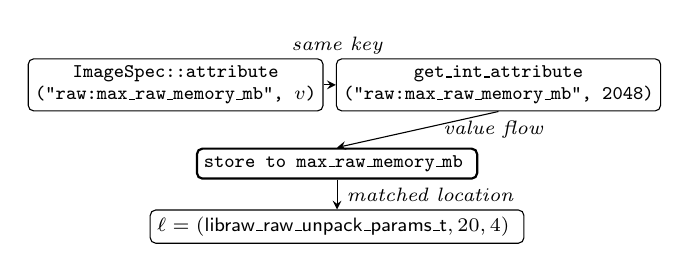
\begin{tikzpicture}[
  font=\scriptsize,
  box/.style={
    draw,
    rounded corners=2pt,
    align=center,
    inner sep=2.5pt
  },
  op/.style={
    draw,
    thick,
    rounded corners=2pt,
    align=center,
    inner sep=2.5pt
  },
  note/.style={
    font=\scriptsize\itshape,
    align=center
  }
]

\node[box] (setter) at (-2.05,1.5) {
  \texttt{ImageSpec::attribute}\\
  \texttt{("raw:max\_raw\_memory\_mb", $v$)}
};

\node[box] (getter) at (2.05,1.5) {
  \texttt{get\_int\_attribute}\\
  \texttt{("raw:max\_raw\_memory\_mb", 2048)}
};

\node[op] (store) at (0,0.5) {
  \texttt{store to max\_raw\_memory\_mb}
};

\node[box] (loc) at (0,-0.3) {
  $\ell=(\mathsf{libraw\_raw\_unpack\_params\_t},20,4)$
};

\draw[->,>=stealth,dashed]
  (setter.east) -- (getter.west);

\node[note] at (0,2) {same key};

\draw[->,>=stealth]
  (getter.south) -- (store.north)
  node[midway,right,xshift=2mm,note]{value flow};

\draw[->,>=stealth]
  (store.south) -- (loc.north)
  node[midway,right,note]{matched location};

\end{tikzpicture}

\caption{Configuration-interface identification in the running example.
\sys links the setter and getter by the shared key and traces the value
to the downstream \texttt{store}.}
\label{fig:interface}
\end{figure}

% \begin{figure}[t]
% \centering
% \begin{tikzpicture}[
%   font=\footnotesize,
%   box/.style={
%     draw,
%     rounded corners=2pt,
%     align=center,
%     inner sep=4pt,
%     minimum width=3.1cm
%   },
%   op/.style={
%     draw,
%     thick,
%     rounded corners=2pt,
%     align=center,
%     inner sep=4pt,
%     minimum width=3.1cm
%   },
%   note/.style={
%     font=\scriptsize\itshape,
%     align=center
%   }
% ]

% \node[box] (setter) at (0,3.3) {
%   \texttt{ImageSpec::attribute}\\
%   \texttt{("raw:max\_raw\_memory\_mb", $v$)}
% };

% \node[box] (getter) at (0,2.0) {
%   \texttt{get\_int\_attribute}\\
%   \texttt{("raw:max\_raw\_memory\_mb", 2048)}
% };

% \node[op] (store) at (0,0.7) {
%   \texttt{store} to\\
%   \texttt{max\_raw\_memory\_mb}
% };

% \node[box] (loc) at (0,-0.6) {
%   $\ell=(\mathsf{libraw\_raw\_unpack\_params\_t},20,4)$
% };

% \draw[->,>=stealth,dashed]
%   (setter.south) --
%   node[note,right]{same attribute key}
%   (getter.north);

% \draw[->,>=stealth]
%   (getter.south) --
%   node[note,right]{value flow}
%   (store.north);

% \draw[->,>=stealth]
%   (store.south) --
%   node[note,right]{matched location}
%   (loc.north);

% \end{tikzpicture}

% \caption{Configuration-interface identification in the running example.
% \sys links the setter and getter by the shared attribute key and traces
% the value to the downstream \texttt{store}.}
% \label{fig:interface}
% \end{figure}

\vspace{3px}
\noindent\textbf{Format-encoded value.}
If neither of the previous interfaces is found, \sys considers cases where the value used to update $\ell$ is encoded in an input buffer. It identifies an input-processing function whose parsed value reaches the operation that updates $\ell$. When a unique interface is found, \sys records the corresponding buffer parameter in $I_D(\ell)$. The following example illustrates this interface, where the caller controls $\ell$ through the contents of the input buffer.

% If neither interface is found, \sys considers configuration values encoded in an input buffer. \sys identifies an input-processing function whose parsed value reaches the operation that updates $\ell$. When a unique interface is found, \sys records the corresponding buffer parameter in $I_D(\ell)$.
% The example below illustrates a format-encoded interface:
%If neither of the above interfaces is found, \sys considers values encoded in an input buffer. In this case, the caller does not provide the configuration value through a dedicated parameter or attribute name; instead, the value is produced while the callee parses the input buffer. \sys identifies an input-processing function whose parsed value reaches the operation that updates $\ell$. When a unique interface is identified, \sys records the corresponding buffer parameter in $I_D(\ell)$, allowing the caller to control $\ell$ by constructing the relevant buffer contents.


% \begin{tcolorbox}[
%   colback=gray!8,
%   colframe=gray!35,
%   boxrule=0.4pt,
%   arc=1pt,
%   left=5pt,
%   right=3pt,
%   top=1pt,
%   bottom=1pt
% ]
% \small\ttfamily
% void configure(char *\textcolor{blue!77!black}{buf}) \{\\
% \hspace*{1.5em}\textcolor{red!77!black}{cfg.limit} = parse(\textcolor{blue!77!black}{buf}); \quad \textcolor{citegray}{// $\ell$}\\
% \}\\
% configure(\textcolor{blue!77!black}{input}); \quad \textcolor{citegray}{// caller}
% \end{tcolorbox}

\begin{tcolorbox}[
  colback=gray!8,
  colframe=gray!35,
  boxrule=0.4pt,
  arc=1pt,
  left=5pt,
  right=3pt,
  top=1pt,
  bottom=1pt
]
\small\ttfamily
void configure(char *\textcolor{blue!77!black}{buf}) \{\\\hspace*{1.5em}\textcolor{red!77!black}{cfg.limit} = parse(\textcolor{blue!77!black}{buf}); \;\textcolor{citegray}{// $\ell$}\\ \} \textcolor{citegray}{// caller invokes configure(input)}
%configure(\textcolor{blue!77!black}{input}); \quad 
\end{tcolorbox}



\begin{algorithm}[t]
    \caption{\small \label{alg:p2}Downstream Configuration Recovery}\small
    \DontPrintSemicolon
    {\footnotesize
    \KwIn{Downstream $D$, upstream paths $\Pi_U$, abstract locations $L_U$}
    \KwOut{Downstream configuration specification $\mathcal{S}$}}
    \SetInd{0.8em}{0.8em}
    \SetKwBlock{Begine}{procedure}{end procedure}
    \BlankLine
    \Begine($\textcolor{red!77!black}{\text{\textsc{\textbf{RecoverDownConfig}}}} {\big(}D, \Pi_U, L_U{\big)}$){
        {$O_D \gets \texttt{FindCandidateOperations}(D, L_U)$\tcp*[r]{$\S$3.2.1}}
        {$O_D \gets \texttt{ClassifyOperations}(O_D, \Pi_U)$\tcp*[r]{$\S$3.2.2}}
        {$\Pi_D \gets \varnothing, R_D \gets \varnothing, I_D \gets \varnothing$\\}        
        \For{$o \in O_D$}{
            {$\pi_D \gets \texttt{RecoverReachablePath}(D, o)$\tcp*[r]{$\S$3.2.3}}
            {\textbf{if} $\pi_D = \varnothing$ \textbf{then continue}\\}   
            {$R_D \gets R_D \cup \texttt{MatchedLocation}(o)$\tcp*[r]{$\S$3.2.3}}
            {$\Pi_D \gets \Pi_D \cup \{\pi_D\}$}
            {$I_D \gets I_D \cup \texttt{IdentifyInterfaces}(o, \pi_D)$\tcp*[r]{$\S$3.2.4}}
        }
        \Return{$\mathcal{S} = (R_D, I_D, \Pi_D, \Pi_U)$}
    }
\end{algorithm}
\normalsize



\PP{Output of P2}
\sys outputs the recovered downstream configuration specification as $\mathcal{S}=(R_D,\,I_D,\,\Pi_D,\,\Pi_U)$, where $R_D$ contains the vulnerability-relevant locations associated with reachable downstream configuration operations, $I_D$ denotes the configuration interfaces recovered for these locations, and $\Pi_D$ and $\Pi_U$ the corresponding downstream and upstream execution paths.
% \sys outputs the recovered downstream configuration specification as $\mathcal{S}=(R_D,\,I_D,\,\Pi_D,\,\Pi_U),$
% where $R_D$ contains reachable vulnerability-relevant locations, $I_D$ their controllable interfaces, and $\Pi_D$ and $\Pi_U$ the corresponding downstream and upstream execution paths. %P3 uses $\mathcal{S}$ to synthesize and validate a concrete vulnerability
%trigger.


% \PP{Output of P2}
% Finally, \sys summarizes the recovered downstream configuration context
% as
% \[
% \mathcal{S}=(R_D,\,I_D,\,\Pi_D,\,\Pi_U),
% \]
% where $R_D$ contains the vulnerability-relevant locations associated with reachable downstream configuration operations, $I_D$ records the corresponding controllable interfaces, and $\Pi_D$ and $\Pi_U$ contain the downstream and upstream execution paths connecting the configuration context to the vulnerability. This specification is used in P3 to synthesize and validate a concrete vulnerability trigger. 

% where $R_D$ contains the vulnerability-relevant locations
% associated with reachable downstream configuration operations,
% $I_D$ records the corresponding controllable interfaces,
% and $\pi_D$ and $\pi_U$ capture the downstream and upstream execution
% paths connecting the configuration context to the vulnerability.
% This specification is used in P3 to synthesize and validate a concrete
% vulnerability trigger.



% \PP{Direct argument.}
% \sys first checks whether the value is exposed through an argument of a public downstream function or boundary API. \sys traces value flow from formal and variadic arguments to the operation that updates $\ell$, including flows through assignments, casts, and intervening calls. When such a flow is found, \sys records the corresponding argument in $\mathit{Iface}(\ell)$.

% \PP{Named-attribute setter.}
% When no direct-argument interface is found, \sys considers generic attribute interfaces that receive a name--value pair. \sys identifies a setter with a compile-time constant attribute name and matches it with a getter in the same class that uses the same name and whose returned value reaches the operation that updates $\ell$. A mapping is accepted only when a unique setter--getter pair is identified, and the setter's value parameter is recorded in $\mathit{Iface}(\ell)$.

% \PP{Format-encoded value.}
% If neither of the above interfaces is found, \sys considers values encoded in an input buffer. \sys identifies an input-processing function whose parsed value reaches the operation that updates $\ell$. When a unique interface is identified, the corresponding buffer parameter is recorded in $\mathit{Iface}(\ell)$.

%\vspace{4px}
% Our running example illustrates the named-attribute case. \sys links \texttt{ImageSpec::\allowbreak attribute} to \texttt{get\_\allowbreak int\_\allowbreak attribute} through the same attribute key \texttt{raw:max\_\allowbreak raw\_\allowbreak memory\_\allowbreak mb} and traces the retrieved value to the downstream \texttt{store} that updates
% $\ell=(\mathsf{libraw\_raw\_unpack\_params\_t},20,4)$. This establishes that the value parameter $v$ of \texttt{ImageSpec::attribute} can reach $\ell$; thus, $v \leadsto_D \ell$, and \sys records $v$ in $\mathit{Iface}(\ell)$.


\subsection{Trigger Synthesis}
Given $\mathcal{S}$, \sys
determines whether the recovered configuration can be concretely
exercised to trigger the vulnerability.

% Although P2 identifies the
% relevant downstream state, interfaces, and execution paths, these
% results remain an abstract specification and do not establish that the
% configuration is feasible in a real execution.


% Given the configuration specification $\mathcal{S}=(C_{\mathrm{drv}},\mathit{Iface},\pi_D,\pi_U)$ recovered in P2 and the PoC $P$, \sys now determines whether the recovered configuration context can be concretely exercised to trigger the vulnerability. 

% To this end, \sys first synthesizes an executable test harness from $\mathcal{S}$ and then searches for concrete configuration values and validates the resulting executions.

% Given the configuration specification $\mathcal{S}=(R_D,I_D,\Pi_D,\Pi_U)$ recovered in P2 and the PoC $P$, \sys now determines whether the recovered configuration context can be concretely exercised to trigger the vulnerability. %P3 consists of test-harness synthesis, configuration value search, and concrete validation.


% The results of P2 specify how a caller can reach the relevant downstream operations and, for Types~1 and~2, which interfaces can supply their values. However, this information remains an abstract specification rather than executable code. Therefore, 

\subsubsection{Synthesizing a Test Harness}\label{subsubsec:harness}
For each recovered path $\pi_D \in \Pi_D$, \sys synthesizes an executable test harness that establishes the downstream configuration along $\pi_D$ and delivers the PoC to $U$. The harness consists of \textit{stubs} that implement the required downstream lifecycle and a \textit{driver} that invokes them, supplies the recovered configuration values, and delivers the PoC.


% For each recovered path $\pi_D \in \Pi_D$, \sys first translates the corresponding configuration specification into an executable test harness that follows $\pi_D$ and delivers the PoC to the upstream component.
% % \sys first translates $\mathcal{S}$ into an executable test harness that follows the recovered path $\pi_D$ and delivers the PoC to the upstream component.

% The test harness consists of a set of \textit{stubs} and a \textit{driver}. The stubs implement the downstream lifecycle needed to exercise the recovered execution path, while the driver invokes them in order, supplies values through the recovered interfaces, and delivers the PoC. \sys synthesizes both automatically from the IR-level information recovered in P2.
%, without manual harness construction.


\PP{Stub}
\sys generates three stubs for the main lifecycle steps: (1) \textit{open} to create the downstream resource and configuration object, (2) \textit{run} to deliver the PoC through $D$ to $U$, and (3) \textit{close} to release the resource. 
Each stub is derived from $\pi_D$ and $I_D$: $\pi_D$ determines which $D$ API calls each stub issues and in what order, while $I_D$ determines the concrete types of receivers and arguments from the IR type identifiers recorded with each interface entry.

%$\pi_D$ determines the required API calls and their order, while $I_D$ provides the receiver and argument types.

% \sys generates three stubs corresponding to the main lifecycle steps of a downstream library consumer: (1) an \textit{open stub} that creates the $D$ resource handle and configuration object, (2) a \textit{run stub} that passes the PoC through $D$ to $U$, and (3) a \textit{close stub} that tears down the resource handle. Each stub is derived from $\pi_D$ and $I_D$: $\pi_D$ determines which $D$ API calls each stub issues and in what order, while $I_D$ determines the concrete types of receivers and arguments from the IR type identifiers recorded with each interface entry.

\PP{Driver}
The driver supplies configuration values and delivers the PoC. For each Type~1 or Type~2 operation with an unknown value, \sys creates a typed open variable and passes it through the recovered interface, for example,
\begin{verbatim}
int32_t se_cfg_0 = 0;
config.attribute("raw:max_raw_memory_mb", se_cfg_0);
\end{verbatim}
% Here, the open variable \texttt{se\_cfg\_0} is concretized in the next stage. 

For Type~3, no open variable is required; the driver only issues the recovered call at the corresponding position in $\pi_D$. 

The PoC remains concrete and is
passed to the run stub. Open variables are initialized to their default values, which are retained for later validation. The resulting harness links against the actual $D$ and $U$ binaries and is directly executable.

% the driver issues the recovered call at the corresponding position in $\pi_D$. The PoC is loaded as concrete bytes and passed to the run stub. The resulting harness links against the actual $D$ and $U$ binaries and is directly executable. Open variables are initialized to their default values, which are also used as the baseline assignment during causal ablation.

\subsubsection{Searching Configuration Values}\label{subsubsec:confvalue}
Direct symbolic execution over the full harness is impractical because symbolic configuration values can induce repeated path forks throughout $D$ and $U$. Instead, \sys performs \textit{domain-guided symbolic execution}, restricting each open variable to a small set of candidate
values derived from the IR.

Each open variable corresponds to a vulnerability-relevant location $\ell$. \sys derives candidate values for $\ell$ from integer constants appearing in operations that read or write it. For each $\ell$, let $K_\ell$ denote these constants. \sys also includes constants along the def--use chains of formal parameters whose values reach these operations. To reduce the analysis scope, \sys optionally uses \texttt{llvm-extract} to restrict this collection to the call-graph neighborhood of $\pi_D$ and the relevant writers; the extracted bitcode is used only for domain analysis, not as input to KLEE~\cite{cadar2008klee}.


For each $c\in K_\ell$, \sys considers $c-1$, $c$, and $c+1$ to capture different outcomes around the corresponding threshold. The candidate domain is
\[
\mathrm{Dom}(\ell)=
\{0,1\}\cup K_\ell
\cup \bigcup_{c\in K_\ell}\{c-1,c+1\}
\cup \{\text{all-ones}\},
\]
where arithmetic is performed modulo the bit width of $\ell$.

Using these domains, \sys precomputes a bounded list of concrete assignments. It first includes the default assignment, then assignments that change one variable at a time, followed by pairwise combinations.

\sys then makes only the index of this list symbolic in KLEE. Each index selects one concrete assignment, while the configuration values and the PoC remain concrete. This avoids symbolic exploration of configuration-dependent branches and the input-processing paths of $D$ and $U$.

% Using these domains, \sys precomputes a bounded list of concrete assignments, beginning with the default assignment, followed by assignments that modify one variable at a time and then pairs of variables. Rather than making the configuration values symbolic and forking execution at branches that depend on them, \sys makes only the index into this list symbolic in KLEE. Each symbolic index selects one precomputed concrete assignment, while the PoC remains concrete. Consequently, KLEE searches among the IR-derived assignments without symbolically exploring the configuration values or the input-processing paths of $D$ and $U$.

% Direct symbolic execution over the full harness is impractical due to the large joint state space of $D$ and $U$. Instead, \sys derives a small finite domain for each open variable from IR constants associated
% with the vulnerability-relevant state.

% For each abstract location $\ell$, let $K_\ell$ denote the integer constants appearing in IR operations that read or write $\ell$. \sys also includes constants along the def--use chains of formal parameters
% whose values reach these operations. To reduce analysis scope, \sys optionally use \texttt{llvm-extract} to restrict this analysis to the call-graph neighborhood of $\pi_D$ and the relevant writers; the extracted bitcode is used only for domain analysis, not as input to KLEE~\cite{cadar2008klee}.


% Direct symbolic execution over the full harness is impractical due to the large joint state space of $D$ and $U$. Instead, \sys derives a small finite domain for each open variable from IR constants associated
% with the vulnerability-relevant state, focusing the search on values near relevant thresholds.

% Applying symbolic execution directly to the full harness is impractical because the large number of branches in $D$ and $U$ would require exploring a large joint state space before reaching the vulnerability.

% To avoid this cost, \sys derives a small finite domain for each open variable from IR constants associated with its vulnerability-relevant state. These constants capture thresholds that may affect the state, allowing \sys to focus the search on values around their boundaries.

% For each abstract location $\ell$, let $K_\ell$ denote the integer constants appearing in IR operations that read or write $\ell$. \sys also includes constants found along the def--use chains of formal parameters whose values reach these operations. \sys optionally uses \texttt{llvm-extract} to restrict this analysis to the call-graph neighborhood of $\pi_D$ and the relevant writers. The extracted bitcode is used only for domain analysis, not as input to KLEE~\cite{cadar2008klee}.

% For each $c \in K_\ell$, \sys considers $c-1$, $c$, and $c+1$ to capture outcomes around the corresponding threshold:
% \[ 
% \mathit{Dom}(\ell)
% =
% \{0,1\}
% \cup K_\ell
% \cup \bigcup_{c\in K_\ell}\{c-1,c+1\}
% \cup \{\mathsf{all\mbox{-}ones}\},
% \]
% where arithmetic is performed modulo the bit width of $\ell$.

% \autoref{table:domain} summarizes the difference between conventional symbolic execution and our domain-guided search.

% This finite domain changes how \sys explores configuration values compared with conventional symbolic execution:

% \begin{table}[t]
% \renewcommand{\tabcolsep}{2.6mm}
% \caption{\label{table:domain}Conventional vs. domain-guided symbolic execution.}
% \small
% \centering
% \begin{tabular}{lll}
% \hline
% \rule{0in}{2.2ex}&\textbf{Conventional} & \textbf{\sys} \\\hline\hline
% %
% %\begin{tabular}[l]{@{}l@{}}\rule{0in}{2ex}\textbf{Configuration}\\\textbf{values}\end{tabular}
% \rule{0in}{2.2ex}\textbf{Configuration values}
% &Symbolic&\begin{tabular}[l]{@{}l@{}}\rule{0in}{2.1ex}Concrete\\candidates\end{tabular}\\\hline
% %
% %\begin{tabular}[l]{@{}l@{}}\rule{0in}{2ex}\textbf{Search}\\\textbf{choice}\end{tabular}
% \rule{0in}{2.2ex}\textbf{Search choice}
% &\begin{tabular}[l]{@{}l@{}}\rule{0in}{2.1ex}Branch\\conditions\end{tabular}
% &\begin{tabular}[l]{@{}l@{}}\rule{0in}{2.1ex}Symbolic\\assignment index\end{tabular}\\\hline
% %
% \rule{0in}{2.2ex}\textbf{PoC}&Concrete&Concrete\\\hline
% %
% %\begin{tabular}[l]{@{}l@{}}\rule{0in}{2ex}\textbf{Path}\\\textbf{exploration}\end{tabular}
% \rule{0in}{2.2ex}\textbf{Path exploration}
% &\begin{tabular}[l]{@{}l@{}}\rule{0in}{2.1ex}Repeated\\symbolic forks\end{tabular}
% &\begin{tabular}[l]{@{}l@{}}\rule{0in}{2.1ex}Candidate\\assignment only\end{tabular}\\\hline
% \end{tabular}
% \end{table}

% \begin{table}[t]
% \centering
% \caption{Comparison of conventional and domain-guided symbolic execution.}
% \label{tab:domain_search}
% \small
% \begin{tabularx}{\columnwidth}{lXX}
% \toprule
% & \textbf{Conventional} & \textbf{\sys} \\
% \midrule
% Configuration values & Symbolic & Concrete candidates \\
% Search choice & Branch conditions & Symbolic assignment index \\
% PoC & Concrete & Concrete \\
% Path exploration & Repeated symbolic forks & Candidate assignments only \\
% \bottomrule
% \end{tabularx}
% \end{table}

% \begin{itemize}
%     \setlength\itemsep{0.2em}
%     \item \textbf{Conventional symbolic execution:}
%     Treating $\ell$ as unconstrained symbolic input causes execution to fork whenever a branch depends on its value, with subsequent branches further multiplying the explored paths.

%     \item \textbf{Domain-guided symbolic execution:}
%     \sys restricts $\ell$ to assignments in $\mathit{Dom}(\ell)$ and forks only over these IR-derived candidates. Subsequent branches depending on $\ell$ are then evaluated under concrete assignments, avoiding additional symbolic forks.
% \end{itemize}


% \begin{itemize}
%     \setlength\itemsep{0.2em}
%     \item Conventional Symbolic execution: When $\ell$ is symbolic, execution forks whenever a branch depends on its value. Further branches then fork each resulting path, leading to path explosion. 
%     \item Domain-guided Symbolic execution: With $\mathit{Dom}(\ell)$ as defined above, \sys restricts the search to IR-derived candidate assignments instead of treating $\ell$ as an unconstrained symbolic value. The executor therefore forks only over these candidates, avoiding forks at later branches whose outcomes depend on $\ell$.
% \end{itemize}

% Using these domains, \sys precomputes a bounded list of concrete assignments. The list begins with the default assignment, followed by assignments that modify one variable at a time and then pairs of variables.
% %
% \sys makes only an index into this list symbolic in KLEE. Each index selects one concrete assignment, while the PoC remains concrete throughout execution. Thus, KLEE chooses among the precomputed assignments rather than symbolically exploring the configuration values
% or input-processing paths of $D$ and $U$.

% Using these domains, \sys precomputes a bounded list of concrete assignments for the open variables, up to a configurable budget. The list begins with the default assignment, followed by assignments that modify one variable at a time and then pairs of variables.

% \sys then makes only an index into this list symbolic in KLEE. Each index selects one precomputed concrete assignment, while the PoC remains concrete throughout execution. As a result, KLEE only chooses among the precomputed assignments instead of symbolically exploring the configuration values or the input-processing paths of $D$ and $U$.

% Using these domains, \sys precomputes a bounded list of concrete assignments for the open variables, up to a configurable budget. The list begins with the default assignment, followed by assignments that change one variable at a time and then pairs of variables. 

% \sys then makes only the index into this list symbolic in KLEE. Each symbolic index selects one precomputed concrete assignment, while the PoC remains concrete throughout execution. Thus, KLEE does not symbolically explore the configuration values or the input-processing paths of $D$ and $U$, confining the search to the IR-derived candidate
% values.

%For Type~1 and Type~2 operations, \sys searches for concrete values of the open variables that trigger the vulnerability under the PoC. However, simply applying symbolic execution to the entire harness is impractical due to the large number of branches in $D$ and $U$.

%\sys avoids this cost by deriving a small finite domain for each open variable from IR constants related to its vulnerability-relevant state. These constants capture thresholds that may affect the state, allowing \sys to focus on values around their boundaries.

% For each abstract location $\ell$, let $K_\ell$ denote the integer constants collected from IR operations that access $\ell$. \sys also includes constants found along the def--use chains of values supplied to those operations.
% \sys optionally uses \texttt{llvm-extract} to restrict this analysis to the call-graph neighborhood of $\pi_D$ and the relevant writers. The extracted bitcode is used only for domain analysis, not as input to KLEE.

% For each $c \in K_\ell$, \sys considers $c-1$, $c$, and $c+1$ to capture different outcomes around the corresponding threshold. The candidate domain is defined as
% \[
% \mathit{Dom}(\ell)
% =
% \{0,1\}
% \cup K_\ell
% \cup \bigcup_{c\in K_\ell}\{c-1,c+1\}
% \cup \{\mathsf{all\mbox{-}ones}\},
% \]
% where arithmetic is performed modulo the bit width of $\ell$.

% Using the derived domains, \sys first generates a bounded list of concrete assignments for the open variables. The list begins with the default assignment, followed by assignments that change one variable at a time and then pairs of variables.

% \sys then makes only the index of this list symbolic in KLEE. Each symbolic index selects one precomputed concrete assignment, which is used to execute the harness while the PoC remains concrete. Thus, KLEE does not symbolically explore the configuration values or the input-processing paths of $D$ and $U$.

\subsubsection{Validating Vulnerability Triggers}\label{subsubsec:trigger}

Finally, \sys executes each candidate assignment using the synthesized harness linked with AddressSanitizer. A candidate triggers the vulnerability when the sanitizer report matches the expected sink location based on the file basename and line number within a small tolerance.

\sys then performs a causal ablation to confirm that the fault depends on the recovered configuration rather than on the PoC alone. It re-executes the same harness with the PoC unchanged but resets all open variables to their default values. If the fault still occurs, \sys rejects the candidate as PoC-only; otherwise, it accepts the candidate assignment as a valid vulnerability trigger.
%
If no candidate assignment within the search budget satisfies these conditions, \sys reports the trigger as unconfirmed.



% \sys executes each candidate assignment using the synthesized test harness linked with AddressSanitizer. A candidate is considered to trigger the vulnerability when the sanitizer report matches the expected sink location, based on the file basename and line number within a small tolerance.

% \sys then performs a causal ablation to verify that the fault depends on the identified configuration values rather than on the PoC alone. It re-executes the same harness with all open variables reset to their default values while keeping the PoC unchanged. If this execution still reaches the fault, \sys rejects the candidate as PoC-only. Otherwise, the candidate assignment is accepted as a valid vulnerability trigger.

% If no candidate assignment within the search budget satisfies these conditions, \sys reports the trigger as unconfirmed.

% Using these domains, \sys constructs a bounded set of candidate assignments, including a zero baseline, one-dimensional sweeps over each open variable, and pairwise combinations. Rather than making the open variables symbolic, \sys uses KLEE to explore only an index into this candidate set, while the PoC remains concrete.
% This confines symbolic execution to the IR-derived candidate values
% without exploring the input-processing paths of $D$ and $U$.

% For Type~1 and Type~2 operations, the remaining task is to determine concrete values for the open variables such that executing the test harness causes $U$ to reach the vulnerability under the PoC. Naively making all open variables symbolic and applying symbolic execution to the entire harness is impractical, because execution through $D$ and $U$ may involve a large number of branches before reaching the vulnerability.

% For Type~1 and Type~2 operations, \sys next identifies how an external caller can supply the value that reaches the vulnerability-relevant state. Because this value may be exposed through different programming interfaces, \sys examines three forms in order: (1) a direct argument, (2) a named-attribute setter, and (3) a format-encoded value. Each form requires a different analysis to recover the externally controllable value. 

% \PP{Direct argument.}
% \sys first checks whether the configuration value is supplied through a typed argument of a downstream entry point or boundary API. For each candidate function, \sys traces SSA value flow from its formal parameters and identifies an argument whose value reaches the operation associated with the vulnerability-relevant state through assignments, casts, or intervening calls. When such a flow is found, \sys records the corresponding function parameter as the configuration interface.

% \PP{Named-attribute setter.}
% When no direct-argument interface is found, \sys checks whether the configuration value is supplied through a generic attribute-setting interface. Such interfaces typically receive a name--value pair rather than exposing the configuration as a dedicated parameter. \sys identifies a setter whose attribute name is a compile-time constant and
% matches it with a corresponding getter that uses the same name and provides the value that eventually reaches the vulnerability-relevant state. When a unique setter--getter pair is found, \sys records the setter's value parameter as the configuration interface.

% \PP{Format-encoded value.}
% If neither of the above interfaces is found, \sys considers cases where the configuration value is encoded in an input buffer rather than passed as an explicit argument. \sys identifies input-processing functions whose parsed values flow to the operation associated with the vulnerability-relevant state. In this case, the input buffer is recorded as the configuration interface, since an external caller controls the relevant value through the buffer contents.

% \vspace{4px}
% For the running example, \autoref{fig:interface} illustrates how \sys recovers the named-attribute interface for \texttt{max_raw_memory_mb}. \sys matches \texttt{ImageSpec::attribute} with \texttt{get_int_attribute} through the common compile-time key \texttt{raw:max_raw_memory_mb}, and traces the value returned by the getter to the downstream \texttt{store}
% associated with the matched abstract location. Consequently, \sys identifies the value parameter of \texttt{ImageSpec::attribute} as the configuration interface.

% For each recoverable operation, P2 outputs the downstream execution sequence $\pi_D$ together with the recovered configuration interface $\mathit{Iface}$. For Type~3 operations, $\mathit{Iface}$ is omitted because the required configuration is represented solely by the identified invocation in $\pi_D$. These outputs are used by P3 to construct and execute a harness under candidate configuration values.


% \sys first locates the vulnerability sink in the IR using the source location obtained from the PoC execution. It then identifies call paths from the boundary APIs in $B$ to the function containing the sink. Along these paths, \sys collects memory reads that may influence the execution leading to the sink as candidate vulnerability-relevant state.

% ========\\
% The core difficulty in recovering $C_C$ is that its two components---the values $D$ prepares for $U$ and the calling sequence $D$ uses to deliver $P$---are split across independently compiled artifacts.
% No single module contains both the downstream configuration logic and the upstream vulnerable path, so a whole-program analysis over $M_U\cup M_D$ would be required to relate them, incurring path explosion across the full downstream driver and upstream library.
% \sys avoids this by keeping the two sides as separately compiled IR modules and joining corresponding memory accesses at \textit{abstract locations}: compact descriptors derived from the compiled layout that identify the same struct field in both modules without relying on shared source names.
% Given the upstream library $U$, the downstream application $D$, and a sink $s$ in $U$, P1 produces a specification $(C_{\mathrm{drv}},\mathit{Iface},\pi_D,\pi_U)$ that names the controllable state, the interface through which a driver reaches it, and the calling sequences in both modules.
% Algorithm~\ref{alg:configuration-dependency} summarizes these stages; the remainder of this subsection follows them in order.

% \begin{algorithm}[t]
% \small
% \caption{Configuration dependency identification}
% \label{alg:configuration-dependency}
% \begin{algorithmic}[1]
% \Require $M_U$, $M_D$, sink $s$, entries $P_D$
% \Ensure controllable $C_C$: state $C_{\mathrm{drv}}$, interfaces $\mathit{Iface}$, sequences $\pi_D,\pi_U$
% \State $B \leftarrow \mathrm{Export}(U)\cap\mathrm{Import}(D)$
% \State $(G_U,G_D) \leftarrow \textsc{BuildCallGraphs}(M_U,M_D)$
% \State $\pi_U \leftarrow \textsc{CallPath}(G_U,B,s)$
% \State $D_{\mathrm{sink}} \leftarrow \textsc{CollectLocations}(G_U,\pi_U,s)$
% \For{each $\ell\in D_{\mathrm{sink}}$}
%   \State $\mathrm{Dep}_D(\ell)\leftarrow\textsc{MatchDependencies}(M_D,M_U,B,\ell)$
% \EndFor
% \State $C(s)\leftarrow\{\ell\in D_{\mathrm{sink}}\mid\mathrm{Dep}_D(\ell)\neq\emptyset\}$
% \State $C_{\mathrm{drv}}\leftarrow\textsc{FilterControllable}(C(s),\mathrm{Dep}_D,P_D)$
% \State $(\mathit{Iface},\pi_D)\leftarrow\textsc{ExtractInterfaces}(M_D,C_{\mathrm{drv}},P_D)$
% \State \textbf{return} $(C_{\mathrm{drv}},\mathit{Iface},\pi_D,\pi_U)$
% \end{algorithmic}
% \end{algorithm}

% \PP{Identifying Boundary APIs}
% \sys first identifies where $D$ calls into $U$, since only calls that cross this boundary can carry or induce configuration changes.
% Let $\mathrm{Export}(U)$ be the functions exported by $U$, and $\mathrm{Import}(D)$ the external callees referenced by $D$.
% Weak and link-once symbols, such as STL inlines, are discarded.
% The boundary is their intersection:
% \begin{equation}
% B \leftarrow \mathrm{Export}(U)\cap\mathrm{Import}(D).
% \label{eq:boundary}
% \end{equation}
% We write $B$ for this set of upstream functions that the downstream application actually invokes, and $P_D$ for the public entries of $D$---the externally visible definitions of $M_D$---from which a driver can later force a configuration.
% On each module, subsequent reachability queries use a call graph with three standard edge kinds: direct callees; indirect callees resolved by Andersen points-to analysis~\cite{sui2016svf}; and callback edges that connect a function-pointer (or vtable) \textit{store} to a later indirect call on the same slot.

% \PP{Identifying Abstract memory locations}
% To relate configuration state across the module boundary, \sys must recognize when a \textit{store} in $D$ and a \textit{load} in $U$ touch the same field---without relying on shared source names.
% Matching by name fails for two structural reasons: the modules do not share named entities (a \textit{store} in $D$ and a \textit{load} in $U$ are never one identifier across compilations), and in IR a field access is a \texttt{getelementptr} with integer indices that denotes a layout slot, not a portable source field name.
% For instance, OpenImageIO stores into \texttt{rawparams.max\_raw\_memory\_mb} after reading the attribute string \texttt{raw:max\_raw\_memory\_mb}, while LibRaw \textit{loads} a field of \texttt{libraw\_raw\_unpack\_params\_t}; neither source name appears in the other module.
% What both sides share is the compiled layout: the aggregate type, the byte offset, and the access width.
% \sys treats that triple as an \textit{abstract memory location}
% \[
% \ell=(\mathsf{agg},\mathsf{off},\mathsf{size})
% \]
% and joins two accesses when these three facts agree.

% \textbf{\emph{Upstream analysis.}}
% The sanitizer report pinpoints $s$ by its source location (file and line).
% \sys resolves this location to IR instructions in $M_U$ through a sequence of fallbacks.
% It first collects every \textit{load} and call instruction whose debug location matches the $s$.
% If none of those instructions is reachable from $B$, \sys falls back to intra-procedural value-flow analysis: it searches the enclosing function for \textit{load} and call instructions whose result flows into the pointer operand of the access at the $s$, since the fault may be reported one program point removed from its root cause.
% If that too yields no reachable candidate, \sys considers call sites within the call-graph path from $B$ to the enclosing function, recovering the case where the reported fault line lies inside a callee not directly invoked from a boundary function.
% In each step, a candidate is retained only if a call-graph path from some boundary function in $B$ to its enclosing function exists, and the corresponding control-flow path within each function on that path reaches the candidate; \sys stops at the first step that produces at least one such candidate.

% Once the candidate set is fixed, \sys collects the abstract locations that the upstream code reads on its way to $s$.
% For each candidate, it walks the call-graph path $\pi_U$ from $B$ to the candidate's enclosing function.
% At each function along $\pi_U$, it gathers every \textit{load} instruction that appears on a control-flow-reachable block from that function's entry to the call site leading to the next function on the path.
% It additionally includes \textit{loads} from the immediate callees of calls on those blocks, without recursing further into the callee tree.
% At an indirect call, only the callee that continues along $\pi_U$ is expanded; other type-compatible targets at the same dispatch site are excluded, since they do not lead to $s$ on this path.
% $D_{\mathrm{sink}}$ is the union of the resulting location sets across all retained candidates.

% For each collected \textit{load}, \sys recovers $\ell$ by walking the \texttt{getelementptr} chain of the pointer operand: when every index is a compile-time constant, it queries the module data layout for the byte offset and access width; a \textit{load} with a runtime-computed index is dropped.
% In Section~\ref{motivating example}, \sys recovers $\ell=(\mathsf{libraw\_raw\_unpack\_params\_t},20,4)$: the four-byte \texttt{max\_raw\_memory\_mb} field at byte offset 20.

% \textbf{\emph{Downstream analysis.}}
% On $M_D$, \sys applies the same constant-\texttt{getelementptr} recovery to every \textit{store} instruction whose destination pointer can be resolved to a compile-time-constant field index, naming each with an abstract location $(\mathsf{agg},\mathsf{off},\mathsf{size})$.
% It likewise records calls to functions in $B$: these are the sites at which a downstream value or invocation may be responsible for updating some $\ell\in D_{\mathrm{sink}}$.

% \textbf{\emph{Joining.}}
% An upstream \textit{load} and a downstream \textit{store} are joined when they resolve to the same $\ell$---the same aggregate, offset, and size---regardless of how each side named the setting in source.
% Figure~\ref{fig:join} illustrates this for Section~\ref{motivating example}.
% Agreeing on layout is necessary but not sufficient for a configuration dependency: unrelated objects may share a layout, and a \textit{store} inside $U$ may execute regardless of what $D$ did.
% The next stage therefore asks how $D$ causes each matched \textit{store}.

% \begin{figure}[t]
% \centering
% \begin{tikzpicture}[
%   font=\footnotesize,
%   mod/.style={draw,rounded corners=2pt,align=center,inner sep=4pt,minimum width=2.9cm},
%   loc/.style={draw,thick,rounded corners=2pt,align=center,inner sep=4pt},
%   note/.style={font=\scriptsize\itshape,align=center}]
% \node[mod] (d) at (-2.4,1.9) {downstream $M_D$\\[2pt]store via\\GEP $i32\,5$};
% \node[mod] (u) at ( 2.4,1.9) {upstream $M_U$\\[2pt]\textit{load} via\\GEP $i32\,5$};
% \node[loc] (l) at (0,0) {$\ell=(\mathsf{libraw\_raw\_unpack\_params\_t},\,20,\,4)$};
% \draw[->,>=stealth] (d.south) -- node[note,right,midway]{layout} (l.north west);
% \draw[->,>=stealth] (u.south) -- node[note,left,midway]{layout} (l.north east);
% \end{tikzpicture}
% \caption{Abstract-location joining in Section~\ref{motivating example}. OpenImageIO stores into \texttt{max\_raw\_memory\_mb} after reading attribute \texttt{raw:max\_raw\_memory\_mb}; LibRaw \textit{loads} a field of \texttt{libraw\_raw\_unpack\_params\_t}. Both compile to the same \texttt{getelementptr} slot (offset~20, size~4), so \sys treats them as one location $\ell$.}
% \label{fig:join}
% \end{figure}

% \PP{Classifying configuration dependencies.}
% A matched abstract location $\ell\in D_{\mathrm{sink}}$ becomes a dependency only when $D$ is the proximate cause of the value observed there.
% The key question is \emph{where the responsible store resides}: if it is in $D$'s own code, $D$ already writes $\ell$ before any boundary call (Type~1); if it is inside $U$, $D$ can only reach it by calling some $F\in B$, and the further question is whether the call argument itself flows into the store (Type~2) or the store fires regardless of what argument is passed (Type~3).
% Types~1 and~2 constitute the \emph{value} component of $C_C$; Type~3 constitutes the \emph{sequence} component.
% When any value-carrying explanation (Type~1 or~2) is present among the matched locations, \sys suppresses Type~3 witnesses entirely: a single supplying store or argument flow is treated as sufficient to explain the configuration, so invocation-only witnesses are not emitted.

% \underline{\emph{Type~1: direct.}}
% $D$ updates $\ell$ in its own code into an object that later crosses $B$, so no specific boundary call is required to establish the value.
% \sys recognizes this when $M_D$ contains a \textit{store} whose destination resolves to $\ell$.
% Constant and read-modify-write \textit{stores} are treated as not introducing a driver-chosen value: they confirm that $D$ touches $\ell$ but do not by themselves displace a Type~3 explanation.
% In Section~\ref{motivating example}, \texttt{max\_raw\_memory\_mb} is written by the keyed setter \texttt{ImageSpec::attribute(\texttt{"raw:max\_raw\_memory\_mb"},$v$)} before the boundary call, and is therefore Type~1.

% \underline{\emph{Type~2: argument-carried.}}
% When the responsible store is inside $U$, $D$ must call $F\in B$ to reach it.
% If the value $D$ passes at that call site is what lands in $\ell$, the dependency is argument-carried.
% \sys checks whether some formal $i$ of $F$ flows into a \textit{store} to $\ell$ in the callee closure of $F$, via ordinary SSA value flow, excluding formals that carry only the address of $\ell$.
% If such an $(F,i)$ exists and $D$ supplies argument $i$ to $F$, \sys records a Type~2 dependency.

% \underline{\emph{Type~3: invocation-induced.}}
% When the store is inside $U$ but no argument flow into $\ell$ can be traced, the act of calling $F$ is itself the configuration: the body of $F$ (transitively) writes $\ell$ regardless of the argument value.
% \sys records this only when no Type~1 or Type~2 explanation applies.
% A call to $F\in B$ qualifies when the callee closure of $F$ contains a \textit{store} to $\ell$ but does \emph{not} contain the sink function, preventing a single opaque library entry from appearing to configure every location the library touches.
% For instance, in the \texttt{libheif}--\texttt{libde265} supply chain, issuing \texttt{heif\_init} transitively initializes the decoder table that \texttt{libde265\_new\_decoder} later reads; nothing is passed to control the outcome, and issuing the call is the configuration.

% We write $\mathrm{Dep}_D(\ell)$ for the witnesses from the three cases, and $C(s)=\{\ell\in D_{\mathrm{sink}}\mid\mathrm{Dep}_D(\ell)\neq\emptyset\}$ for the candidate set.

% \PP{Identifying interfaces and sequences.}
% A candidate location in $C(s)$ is useful only if a driver can actually reach the code that establishes it---it must be triggerable from a public entry point of $D$, not buried in an internal path that the driver cannot invoke.
% \sys checks, for each dependency witness $I\in\mathrm{Dep}_D(\ell)$, whether a call-graph path from a public entry in $P_D$ reaches $I$, following direct calls, indirect calls, and callback edges.
% Let $\mathrm{Reach}_D(P_D,I)$ denote this condition.
% \sys retains only the locations for which at least one witness is reachable:
% \begin{equation}
% C_{\mathrm{drv}}=\{\ell\in C(s)\mid\exists\,I\in\mathrm{Dep}_D(\ell).\ \mathrm{Reach}_D(P_D,I)\},
% \label{eq:driver-state}
% \end{equation}
% and records a witnessing call sequence $\pi_D$---a call-graph path from a public entry to the dependency witness that establishes $\ell$.
% This single reachability check therefore answers two questions at once: whether the configuration is controllable from outside, and what call sequence reaches the responsible site.

% The remaining question is which concrete call---and which of its parameters---the harness must issue to force $\ell$ to a target value.
% In real execution the path is always $D\to U$: a driver calls $D$'s public functions, and $D$ in turn calls $U$ through boundary functions in $B$.
% \sys therefore searches both the public functions of $D$ and the boundary functions in $B$.

% For each candidate function, the core question is: \emph{how does the desired value of $\ell$ reach that function?}
% The answer depends on a two-level distinction.
% At the first level, the value either arrives as an \emph{explicit argument} or is determined \emph{implicitly} by the content of a data buffer that the function parses.
% If the value is explicit, a second question arises: is it carried by a typed parameter that flows directly into $\ell$, or does it reach $\ell$ only after a name-based dispatch inside a generic setter?
% This decomposition yields three cases.
% \sys tries them in priority order---direct argument, then named-attribute setter, then format-encoded value---and installs an interface only when exactly one witness remains (a unique-witness rule).
% Ambiguous candidates are dropped rather than deferred.

% \begin{enumerate}
% \item \textbf{Direct argument.}
% The caller passes the configuration value as a typed argument; the function routes it to $\ell$ through data-flow operations---assignments, casts, or calls, including variadic argument lists.
% Because the mapping from call site to memory location is visible in the function's type signature, the harness controls $\ell$ simply by choosing the value of that argument.
% \sys identifies this case by tracing SSA value flow from each formal of the candidate function to a \textit{store} to $\ell$.

% \item \textbf{Named-attribute setter.}
% The caller supplies a (name,~value) pair to a generic setter, while a paired getter under the same compile-time name supplies the value that $D$ later stores into $\ell$---for example, \texttt{ImageSpec::attribute("raw:max\_raw\_memory\_mb",~$v$)} paired with \texttt{get\_int\_attribute} on the same key.
% Unlike a typed argument, the mapping from name to location is encoded in the getter/setter bodies rather than in a single formal's type.
% \sys identifies this case only when the Direct-argument candidate set is empty, the name is a compile-time string constant, and the getter--setter dual is a unique same-class witness for that name.

% \item \textbf{Format-encoded value.}
% The caller passes a raw data buffer to an input-processing function; $\ell$ is written as a side effect of interpreting that buffer's content, so the field is not addressable by name at the call site.
% The harness controls $\ell$ by crafting the relevant bytes in the buffer rather than by naming a configuration field.
% \sys considers this case only when neither Direct nor Named-attribute candidates exist, and accepts it only under the same unique-witness rule.
% \end{enumerate}

% We write $\mathit{Iface}$ for the set of recovered interface parameters associated with $C_{\mathrm{drv}}$.

% \sys emits $(C_{\mathrm{drv}},\mathit{Iface},\pi_D,\pi_U)$ as the complete specification of $C_C$.
% In Section~\ref{motivating example}, the surviving location is Type~1: $D$ stores into \texttt{max\_raw\_memory\_mb} after reading the named attribute \texttt{raw:max\_raw\_memory\_mb}, and the harness injects that attribute through \texttt{ImageSpec::attribute} along a path reachable from \texttt{ImageInput::open}.
% In the \texttt{libheif}--\texttt{libde265} case, the configuration is Type~3, realized by the call chain \texttt{heif\_init}\,$\rightarrow\cdots\rightarrow$\,\allowbreak\texttt{libde265\_new\_decoder}.

% \PP{Precision.}
% P1 is deliberately permissive and defers every verdict to concrete validation in P2.
% It over-approximates when two unrelated objects share the same abstract location (same aggregate, offset, and size), or when an imprecise indirect or callback edge makes a witness appear reachable along a path the application never takes.
% It under-approximates when a \texttt{getelementptr} index is computed at run time (the \textit{load} is dropped) or when bounded value-flow search misses a longer chain.
% An over-approximated fact costs P2 search budget but is harmless: validation accepts a configuration only when AddressSanitizer observes a fault at the expected sink location under the candidate assignment, and causal ablation rejects cases where the PoC alone is sufficient.
% An under-approximated fact is lost and reported as unconfirmed.

% \subsection{Trigger Synthesis (P2)}
% \label{subsec:p2}

% P1 identifies \emph{what} configuration is needed; P2 determines \emph{whether} that configuration can be concretely realized to reproduce the fault.
% Given $\mathcal{S}=(C_{\mathrm{drv}},\mathit{Iface},\pi_D,\pi_U)$, P2 must produce a test harness that invokes $D$'s interface along $\pi_D$ and a concrete assignment for each open configuration value that causes $U$ to reach the fault at $s$ under the PoC $P$.
% The calling sequence $\pi_D$ is already fully determined by $\mathcal{S}$; the only quantities remaining to be resolved are the value-component unknowns in $C_{\mathrm{drv}}$.
% P2 addresses these in two steps: it first synthesizes a test harness from $\mathcal{S}$, then derives a small domain for each open variable from IR constants, enumerates a bounded set of candidate assignments, and validates each against the live AddressSanitizer-instrumented binary.
% Algorithm~\ref{alg:trigger-synthesis} formalizes these steps.

% \begin{algorithm}[t]
% \small
% \caption{Trigger synthesis}
% \label{alg:trigger-synthesis}
% \begin{algorithmic}[1]
% \Require P1 specification $\mathcal{S}$, PoC $P$, sink $s$
% \Ensure harness $H$ and concrete configuration $c$, or $\bot$
% \State $H \leftarrow \textsc{SynthesizeHarness}(\mathcal{S},P)$
% \State $X \leftarrow \textsc{OpenValues}(\mathcal{S})$
% \For{each $x\in X$}
%   \State $\mathit{Dom}(x) \leftarrow \textsc{DeriveDomain}(x,\mathcal{S})$
% \EndFor
% \State $Q \leftarrow \textsc{EnumerateCandidates}(\{\mathit{Dom}(x)\}, \mathit{budget})$
% \State $T \leftarrow \textsc{IndexSymbolicSearch}(Q)$ \Comment{KLEE over assignment indices}
% \For{each $c\in T$}
%   \If{$\textsc{Validate}(H,P,c,s)$}
%     \State \textbf{return} $(H,c)$
%   \EndIf
% \EndFor
% \State \textbf{return} $\bot$
% \end{algorithmic}
% \end{algorithm}

% \PP{Synthesizing a harness}
% P1 produces a specification $\mathcal{S}=(C_{\mathrm{drv}},\mathit{Iface},\pi_D,\pi_U)$ that names the configuration state, the interfaces to set it, and the calling sequences in both modules---but $\mathcal{S}$ is an abstract description, not executable code.
% The first task of P2 is therefore to translate $\mathcal{S}$ into a compilable C++ program that can run the downstream configuration and deliver $P$ to $U$.
% A test harness consists of two components: \emph{stubs}---generated functions that implement the lifecycle steps of a library consumer---and a \emph{driver}---the \texttt{main} entry point that calls those stubs in order, injects the configuration values, and delivers $P$.
% \sys synthesizes both mechanically from the IR-level information in $\mathcal{S}$, requiring no human authoring.

% \textbf{Stubs.}
% The stubs implement the three lifecycle steps of a library consumer: an \emph{open} stub that creates the $D$ resource handle and configuration object, a \emph{run} stub that passes $P$ through $D$ to $U$, and a \emph{close} stub that tears down the handle.
% Each stub is derived from $\pi_D$ and $\mathit{Iface}$: $\pi_D$ determines which $D$ API calls each stub issues and in what order; $\mathit{Iface}$ determines the concrete types of receivers and arguments from the IR type identifiers recorded with each interface entry.

% \textbf{Driver.}
% The driver ties the stubs together and handles the two remaining tasks: injecting the configuration values and delivering $P$.
% Each value-component unknown---a configuration field for which P1 identified an interface but not a concrete value---appears in the driver as a typed \emph{open variable} declared immediately before the open stub call, for example:
% \begin{center}
% \texttt{int32\_t se\_cfg\_0 = 0; \quad config.attribute("raw:max\_raw\_memory\_mb",\;se\_cfg\_0);}
% \end{center}
% The open variable \texttt{se\_cfg\_0} is the quantity that targeted symbolic execution will concretize in the next stage.
% Sequence-component dependencies (Type~3) require no open variable; the driver simply issues the identified call in the correct position, since the act of calling is itself the configuration.
% $P$ is loaded from disk as concrete bytes and passed to the run stub.

% The resulting harness links against the real $D$ and $U$ binaries and is immediately runnable.
% Open variables are initialized to default values in the emitted source; those defaults also serve as the zero assignment used later for causal ablation.

% \PP{Targeted symbolic execution.}
% The remaining task is to assign concrete values to the open variables so that running the test harness with those values causes $U$ to reach the fault at $s$.
% Making all open variables unconstrained and running KLEE~\cite{267932} on the full harness is impractical: a single entry path through $U$ introduces thousands of branches, and the solver would explore the joint state space of $D$ and $U$ before reaching the relevant fault condition.

% \sys avoids this cost by observing that the open variables are both \emph{few} and \emph{tightly constrained}.
% Each open variable corresponds to a specific configuration field $\ell$ whose exploitability effect is decided by comparisons against integer constants that already appear in the IR of the writers and readers of $\ell$.
% For each such constant $c$, the neighboring values $c-1$, $c$, and $c+1$ capture the distinct outcomes around that threshold.
% \sys therefore derives a small finite domain for each open variable and searches only over those values.

% Concretely, for each $\ell\in C_{\mathrm{drv}}$, \sys collects integer constants from the IR that writes or reads $\ell$---including constants on the def--use chains of supplying formals and constants that appear at accesses to the matched abstract location---into $K_\ell$.
% Optional \texttt{llvm-extract} focuses this scrape on the call-graph neighborhood of $\pi_D$ and the writers of $C_{\mathrm{drv}}$, but the extracted bitcode is used only for domain analysis, not as the KLEE input module.
% The value domain is then
% \begin{equation}
% \mathrm{Dom}(\ell)=\{0,1\}\cup K_\ell\cup\bigcup_{c\in K_\ell}\{\,c-1,\;c+1\,\}\cup\{\mathit{all\text{-}ones}\},
% \label{eq:value-domain}
% \end{equation}
% with arithmetic modulo the width of $\ell$.
% In the motivating example, constants around the overflow-guard threshold on the vulnerable path collapse the $2^{32}$-value space of \texttt{raw:max\_raw\_memory\_mb} to a handful of candidate values.

% With the domains fixed, \sys does \emph{not} ask KLEE to solve for open variables inside the library IR.
% Instead it precomputes a bounded list of candidate assignments---a zero baseline, one-dimensional sweeps over each open variable's domain, then pairwise combinations---up to a configurable budget.
% KLEE explores only an index into this list, while $P$ remains concrete throughout the subsequent AddressSanitizer replay.
% This keeps symbolic execution outside $U$'s input-processing path and confines the search to the IR-derived candidate values.

% Each assignment that KLEE selects by index is replayed in the test harness linked against AddressSanitizer.
% \sys accepts a candidate when the sanitizer report matches the expected sink location (file basename and line, within a small tolerance).
% To check that the fault depends on the identified configuration rather than on $P$ alone, \sys then performs a causal ablation: it re-runs the harness once with \emph{all} open variables reverted to their default (zero) values.
% If that ablated run still faults, the candidate is classified as PoC-only and rejected as a configuration trigger; if only the winning assignment faults, the dependency is confirmed as causal.
% If no assignment within the budget is accepted, \sys reports the dependency as unconfirmed.

% \begin{figure}[t]
% 	%\vspace{-0.5em}

% 	\begin{center}
% 		\begin{subfigure}[b]{0.23\textwidth}
% 			\centering
% 			\includegraphics[width=\linewidth]{./imgs/con_se.pdf}
	
% 			\vspace{-0.3em}
% 			\caption{Conventional}
% 			\label{fig:con_se}
% 		\end{subfigure}\hspace{0.0em}%
% 		\begin{subfigure}[b]{0.23\textwidth}
% 			\centering
% 			\includegraphics[width=\linewidth]{./imgs/con_sys.pdf}
			
% 			\vspace{-0.3em}
% 			\caption{\sys}
% 			\label{fig:con_sys}
% 		\end{subfigure}
		  
% 		\caption{SIMDIFF.}\label{fig:sym_diff}
% 	\end{center}
% \end{figure}

% \begin{figure}[t]
%   \centering
%   \fbox{\begin{minipage}[c][1.15in][c]{0.95\columnwidth}
%     \centering\small Figure placeholder\\[0.3em]
%   \end{minipage}}
%   \caption{Search scope of conventional symbolic execution and of \sys.}
%   \label{fig:scope}
% \end{figure}


% \PP{Overview}
% \textcolor{blue}{\autoref{fig:pipeline} shows the high-level workflow of \sys, which comprises two phases: P1 for \textit{cross-layer condition reconstruction} and P2 for \textit{configuration validation}.}

% \textcolor{blue}{Given a PoC that supplies the \textit{data context}, \sys attempts to recover the \textit{configuration context}. In P1, \sys.... In P2, \sys .... The output is ....}
 
% % % 파란글자들은 comment 확인
% % \textcolor{blue}{In this section, we describe the design of \sys, a precise approach for statically assessing upstream vulnerability exploitability by recovering the configuration context required by a given data context.}

% % \PP{Overview}
% % \textcolor{blue}{\autoref{fig:pipeline} shows the high-level workflow of \sys, which comprises two phases: P1 for \textit{cross-layer condition reconstruction} and P2 for \textit{configuration validation}.}

% % \textcolor{blue}{Given a PoC that supplies the \textit{data context}, \sys attempts to recover the \textit{configuration context}. In P1, \sys.... In P2, \sys .... The output is ....}

% \PP{Preliminary concepts.}
% \textcolor{blue}{Exploitability depends on two independent context (see \autoref{subsubsec:cond}).}

% \begin{itemize}
%     \item \textcolor{blue}{The \textit{data context} is the payload delivered to the vulnerability sink and is provided by the given PoC $P$.}

%     \item  \textcolor{blue}{ The \textit{configuration context} is the program state established by the downstream driver and libraries before control reaches the upstream component $U$.}
% \end{itemize}

% \textcolor{blue}{The two contexts are independent: the data context determines which bytes reach the sink, whereas the configuration context determines the internal state under which those bytes are processed. Because the data context is already provided by $P$, \sys focuses on recovering the configuration context required to trigger the vulnerability. This requires relating state established in the downstream layer to state consumed in the upstream layer.}

% \textcolor{blue}{We formalize this relation using three concepts: \circled{1} \textit{boundary APIs} identify where control and state cross the layer boundary, \circled{2} \textit{abstract locations} provide a layer-independent representation of shared state, and \circled{3} environment settings identify the shared locations whose values are externally controllable.}

% \vspace{4px}
% \noindent\textbf{Definition \circled{1}: Boundary API.} Given...

% === 

